\documentclass[11pt,oneside]{article}

\usepackage[a4paper,margin=26mm,headheight=14pt]{geometry}
\usepackage[T1]{fontenc}
\usepackage[utf8]{inputenc}
\usepackage{lmodern}
\usepackage{microtype}
\usepackage{amsmath,amssymb,amsthm,mathtools}
\usepackage{booktabs,longtable,array,tabularx}
\usepackage{enumitem}
\usepackage{xcolor}
\usepackage{hyperref}
\usepackage{cleveref}
\usepackage{listings}
\usepackage{fancyhdr}
\usepackage{tikz}
\usetikzlibrary{arrows.meta,positioning,fit}

\definecolor{leanblue}{HTML}{0B4F8A}
\definecolor{darkgreen}{HTML}{246B45}
\definecolor{brick}{HTML}{8B2E2E}
\definecolor{lightblue}{HTML}{EEF6FC}
\definecolor{lightamber}{HTML}{FFF7E5}
\definecolor{lightgray}{HTML}{F4F5F7}

\hypersetup{
  colorlinks=true,
  linkcolor=leanblue,
  citecolor=darkgreen,
  urlcolor=leanblue,
  pdftitle={A Self-Contained Lean Blueprint for the Evans--Hrushovski--Gismatullin Reconstruction Theorem},
  pdfauthor={Self-contained formalization blueprint prepared for Mathlib}
}

\pagestyle{fancy}
\fancyhf{}
\lhead{Field reconstruction from algebraic-dependence geometry}
\rhead{Lean/Mathlib blueprint}
\cfoot{\thepage}

\newtheorem{theorem}{Theorem}[section]
\newtheorem{lemma}[theorem]{Lemma}
\newtheorem{proposition}[theorem]{Proposition}
\newtheorem{corollary}[theorem]{Corollary}
\theoremstyle{definition}
\newtheorem{definition}[theorem]{Definition}
\newtheorem{construction}[theorem]{Construction}
\newtheorem{milestone}[theorem]{Milestone}
\theoremstyle{remark}
\newtheorem{remark}[theorem]{Remark}
\newtheorem{warning}[theorem]{Warning}

\newcommand{\acl}{\operatorname{acl}}
\newcommand{\trdeg}{\operatorname{trdeg}}
\newcommand{\cl}{\operatorname{cl}}
\newcommand{\Aut}{\operatorname{Aut}}
\newcommand{\Frob}{\operatorname{Frob}}
\newcommand{\rk}{\operatorname{rk}}
\newcommand{\Perf}{\operatorname{Perf}}
\newcommand{\RAC}{\operatorname{RAC}}
\newcommand{\G}{\mathcal{G}}
\newcommand{\Ga}{\mathbb G_{\mathrm a}}
\newcommand{\Gm}{\mathbb G_{\mathrm m}}
\newcommand{\Loc}{\operatorname{Loc}}
\newcommand{\Stab}{\operatorname{Stab}}
\newcommand{\Qrel}{\mathcal{Q}}
\newcommand{\Qprel}{\mathcal{Q}'}
\newcommand{\Jrel}{\mathcal{J}}
\newcommand{\Set}{\mathsf{Set}}
\newcommand{\Prop}{\mathsf{Prop}}
\newcommand{\Type}{\mathsf{Type}}
\newcommand{\lean}[1]{\nolinkurl{#1}}

\newcommand{\statusmathlib}{\textcolor{darkgreen}{\textbf{Mathlib}}}
\newcommand{\statusnew}{\textcolor{brick}{\textbf{new}}}
\newcommand{\statusglue}{\textcolor{leanblue}{\textbf{glue}}}

\lstdefinelanguage{Lean}{
  morekeywords={universe,variable,namespace,end,def,abbrev,structure,class,where,
    theorem,lemma,instance,noncomputable,section,open,scoped,if,then,else,match,
    with,let,in,by,fun,forall,exists,Prop,Type,Set,Field,Algebra},
  sensitive=true,
  morecomment=[l]{--},
  morecomment=[s]{/-}{-/},
  morestring=[b]"
}
\lstset{
  language=Lean,
  basicstyle=\ttfamily\small,
  keywordstyle=\color{leanblue}\bfseries,
  commentstyle=\color{darkgreen},
  stringstyle=\color{brick},
  columns=fullflexible,
  keepspaces=true,
  showstringspaces=false,
  frame=single,
  framerule=0.3pt,
  rulecolor=\color{gray!50},
  backgroundcolor=\color{lightgray},
  breaklines=true,
  xleftmargin=4pt,
  xrightmargin=4pt
}

\newenvironment{resultbox}
  {\par\medskip\begin{center}\begin{minipage}{0.94\linewidth}\color{leanblue}\hrule\medskip\color{black}}
  {\medskip\color{leanblue}\hrule\end{minipage}\end{center}\par\medskip}
\newenvironment{riskbox}
  {\par\medskip\begin{center}\begin{minipage}{0.94\linewidth}\color{brick}\hrule\medskip\color{black}}
  {\medskip\color{brick}\hrule\end{minipage}\end{center}\par\medskip}

\title{\bfseries A Self-Contained Formalization Blueprint for the\\
Evans--Hrushovski--Gismatullin Reconstruction Theorem\\[4pt]
\large Complete specialized proofs for reconstruction from algebraic-dependence geometry in Lean 4 and Mathlib}
\author{Technical proof and implementation blueprint}
\date{Mathlib API audit: 5 August 2026}

\begin{document}
\maketitle

\begin{abstract}
This document is a self-contained, implementation-level blueprint for formalizing the theorem that a
relatively algebraically closed field extension of transcendence degree at least five is
determined, up to perfection, by its full algebraic matroid (equivalently, by the complete
lattice of relatively algebraically closed intermediate fields).  It states the theorem in
a Lean-friendly form, corrects three often-omitted qualifications, separates the parts already
available in Mathlib from the new mathematics, gives exact predicates for the finite
configurations used by Evans--Hrushovski and Gismatullin, and specifies the quotient
construction which interprets the perfect closure as a field.  Every mathematical result
not already present in Mathlib is proved below.  In particular, the general machinery of
stability theory is replaced by a proof of the one algebraic group--configuration statement
actually used here, phrased entirely in terms of irreducible loci, transcendence degree,
finite correspondences, and rational group chunks.  The additive and multiplicative
correspondence theorems, simultaneous Frobenius rigidity, the $21$-point calculation,
Gismatullin transfer, generic totalization, base recovery, point recovery, and the
Frobenius kernel all receive complete proofs.  The final sections also construct the
geometry functor, prove its identity and composition laws, determine every Hom-set fibre,
and prove the corrected fully faithful assertion after quotienting source morphisms by
integral Frobenius.  Lean fragments record target interfaces; the prose proofs immediately
preceding them are the proofs to be transcribed.
\end{abstract}

\begin{resultbox}
\textbf{Three corrections to the informal statement.}
The theorem requires $\trdeg(K/k)\geq 5$.  Moreover, in characteristic $p>0$ the
perfect-closure isomorphism inducing a prescribed geometry isomorphism is not literally
unique: it is unique modulo composition with an integral power of Frobenius.  In
characteristic zero it is genuinely unique.  Consequently, with actual perfect-field
isomorphisms as arrows, the geometry functor is not faithful in positive characteristic:
the identity and Frobenius are distinct arrows with the same image.  The fully faithful
statement is true either in characteristic zero or after quotienting every source Hom-set
by integral Frobenius.  These are parts of the theorem, not merely artifacts of the proof.
\end{resultbox}

\tableofcontents
\newpage

\section{The exact mathematical target}

\subsection{Geometric lattice and combinatorial geometry}

Let $k\subseteq K$ be a field extension and assume that $k$ is relatively algebraically
closed in $K$.  Write
\[
  \G(K/k)=\{M: k\subseteq M\subseteq K\mid M\text{ is relatively algebraically closed in }K\}.
\]
Ordered by inclusion, this is a complete lattice.  Its infima are intersections, and the
supremum of $(M_i)_i$ is the relative algebraic closure in $K$ of the compositum of the
$M_i$.

The associated combinatorial geometry has as points the atoms of $\G(K/k)$, equivalently
the relatively algebraically closed intermediate fields of transcendence degree one.  If
$S$ is a set of atoms, then
\[
  \cl(S)=\{P\text{ atom}:P\leq \bigvee S\}.
\]
Conversely, $\G(K/k)$ is canonically isomorphic to the lattice of closed subsets of this
point geometry.  Thus an isomorphism of either presentation functorially determines an
isomorphism of the other.  The lattice-first presentation is recommended in Lean: it
avoids quotient representatives in the theorem statement and makes the final extension
from points to all closed subextensions automatic.

\subsection{Correct reconstruction theorem}

For a field $F$, let $F^{\mathrm{perf}}$ denote a chosen perfection.  If the characteristic
exponent is $p$ (so $p=1$ in characteristic zero), the notation $x\mapsto x^{p^n}$ for
$n\in\mathbb Z$ means the $n$th integral iterate of Frobenius on the perfect field.

\begin{theorem}[Evans--Hrushovski--Gismatullin, lattice form]\label{thm:target}
Let $K/k$ and $L/l$ be relatively algebraically closed field extensions, and suppose
$\trdeg(K/k)\geq5$.  If
\[
  \phi:\G(K/k)\overset{\sim}{\longrightarrow}\G(L/l)
\]
is an order isomorphism, then $\trdeg(L/l)=\trdeg(K/k)$ and there is a field isomorphism
\[
  \Phi:K^{\mathrm{perf}}\overset{\sim}{\longrightarrow}L^{\mathrm{perf}}
\]
such that $\Phi(k^{\mathrm{perf}})=l^{\mathrm{perf}}$ and, for every
$M\in\G(K/k)$,
\[
  \phi(M)=\Phi(M^{\mathrm{perf}})\cap L.
\]
If $\Phi_1$ and $\Phi_2$ induce the same $\phi$, then
\[
  \Phi_2=\Frob_{L^{\mathrm{perf}}}^{,n}\circ\Phi_1
\]
for some $n\in\mathbb Z$.  If $p=1$, then $\Phi_1=\Phi_2$.  If $p>1$, the integer $n$
is unique.  Conversely, any perfect-field isomorphism carrying $k^{\mathrm{perf}}$ onto
$l^{\mathrm{perf}}$ induces such a lattice isomorphism.
\end{theorem}

This is the form stated explicitly in Topaz~\cite[Theorem 4.4]{Topaz2022}, deduced from
Gismatullin~\cite[Theorem 4.2]{Gismatullin2008} and the earlier work of
Evans--Hrushovski~\cite{EH1991,EH1995}.  Gismatullin states both extensions with
transcendence degree at least five.  In the lattice formulation it suffices to assume this
on one side, because a lattice isomorphism preserves the cardinal rank; the first Lean
version should assume it on both sides and derive the one-sided wrapper afterwards.

\subsection{A type-correct statement should not choose incompatible perfections}

The concrete type \lean{PerfectClosure K p} in Mathlib is most convenient in positive
prime characteristic.  A theorem covering characteristic zero and positive characteristic
uniformly should instead quantify over chosen target fields and embeddings satisfying
\lean{IsPerfectClosure}.  A useful project-local bundle is:

\begin{lstlisting}
-- Interface sketch; universe/typeclass details must be adjusted in Lean.
structure Perfection (F : Type u) [Field F] where
  carrier : Type v
  [fieldCarrier : Field carrier]
  expChar : Nat
  [expCharF : ExpChar F expChar]
  [expCharCarrier : ExpChar carrier expChar]
  incl : F ->+* carrier
  [perfectCarrier : PerfectRing carrier expChar]
  [isPerfectClosure : IsPerfectClosure incl expChar]
\end{lstlisting}

For an intermediate field $M$ of $K/k$, define $M^{\mathrm{perf}}$ as a \lean{Subfield}
of the chosen perfection of $K$.  Its main API theorem should be the membership criterion
\[
 x\in M^{\mathrm{perf}}
 \quad\Longleftrightarrow\quad
 \exists n\in\mathbb N\ \exists m\in M,
 x^{p^n}=\iota_K(m).
\]
In characteristic zero this reduces to membership in the image of $M$.  Define
\lean{Induces phi Phi} by the equality of perfected subfields
\[
  (\phi M)^{\mathrm{perf}}=\Phi(M^{\mathrm{perf}})
  \qquad(M\in\G(K/k)).
\]
This is type-clean, implies the displayed intersection formula in
\cref{thm:target}, and includes the base condition by applying it to the bottom element.

\section{What may be taken from Mathlib}

The following audit is deliberately conservative.  ``Mathlib'' means that the main
object or theorem is present; nontrivial adapter lemmas may still be needed.  ``New''
means that the result must be proved in the project---a citation to the papers is not an
acceptable Lean axiom.

\begin{longtable}{>{\raggedright\arraybackslash}p{0.29\linewidth}
                  >{\raggedright\arraybackslash}p{0.13\linewidth}
                  >{\raggedright\arraybackslash}p{0.49\linewidth}}
\toprule
Component & Status & Relevant API or required work\\
\midrule
\endfirsthead
\toprule
Component & Status & Relevant API or required work\\
\midrule
\endhead
Relative algebraic closure & \statusmathlib &
\lean{algebraicClosure F E}, \lean{mem_algebraicClosure_iff}, map/comap lemmas,
and \lean{algebraicClosure.algebraicClosure_eq_bot} are in
\lean{Mathlib.FieldTheory.AlgebraicClosure}.\\
Intermediate fields & \statusmathlib &
\lean{IntermediateField.adjoin}, map, comap, restriction of scalars, and the complete
lattice of intermediate fields are available.\\
Algebraic independence and transcendence degree & \statusmathlib &
\lean{AlgebraicIndependent}, \lean{AlgebraicIndepOn}, transcendence bases, and
\lean{Algebra.trdeg} are available in the algebraic-independence and field-theory files.\\
Perfect closures and Frobenius & \statusmathlib &
\lean{perfectClosure}, \lean{mem_perfectClosure_iff_pow_mem},
\lean{IsPerfectClosure}, \lean{PerfectRing.lift},
\lean{IsPerfectClosure.equiv}, and \lean{iterateFrobeniusEquiv} supply the basic
perfection API.\\
General matroids & \statusmathlib &
Mathlib has infinite matroids and closure theory.  There is no audited, ready-made
constructor identifying algebraic independence with a \lean{Matroid} on this quotient.
The project can use a small purpose-built geometry API first and add a matroid instance
later.\\
First-order syntax & \statusmathlib &
\lean{Mathlib.ModelTheory.Basic} provides languages, structures, formulas, and maps.
No ACF stability theory or group-configuration theorem needed here is available.\\
Closed-subextension lattice & \statusnew &
Define the fixed points of relative algebraic closure, construct their complete lattice,
and prove atomisticity.\\
Geometry/lattice equivalence & \statusnew &
Atoms, point closure, exchange, and the equivalence with the lattice of closed point sets.\\
Perfection invariance of the lattice & \statusnew &
Map a closed $M$ to $M^{\mathrm{perf}}$ and invert by intersection/comap.\\
Finite configuration predicates & \statusnew &
The predicates $\Qrel,\Qprel,\Jrel$, the $21$-point witness, multiplication diagram,
Frobenius-link relation, and generic arithmetic.\\
One-quantifier transfer & \statusnew &
Only the specialized closure-membership transfer used by Gismatullin is needed.\\
Algebraic-correspondence rigidity & \statusnew &
This is the hard core: additive and multiplicative correspondences, simultaneous
Frobenius rigidity, and correctness of the Evans--Hrushovski configurations.\\
Interpreted ratio field & \statusnew &
Setoids and quotient infrastructure are in Mathlib; all geometric well-definedness and
naturality results are new.\\
Kernel/uniqueness theorem & \statusnew &
Show that an automorphism acting trivially on the geometry is an integral Frobenius
power.\\
\bottomrule
\end{longtable}

The relevant generated documentation includes
\href{https://leanprover-community.github.io/mathlib4_docs/Mathlib/FieldTheory/AlgebraicClosure.html}{relative algebraic closure},
\href{https://leanprover-community.github.io/mathlib4_docs/Mathlib/FieldTheory/PurelyInseparable/PerfectClosure.html}{relative perfect closure},
\href{https://leanprover-community.github.io/mathlib4_docs/Mathlib/FieldTheory/IsPerfectClosure.html}{abstract perfect closures},
\href{https://leanprover-community.github.io/mathlib4_docs/Mathlib/RingTheory/AlgebraicIndependent/Basic.html}{algebraic independence}, and
\href{https://leanprover-community.github.io/mathlib4_docs/Mathlib/Combinatorics/Matroid/Basic.html}{matroids}.

\begin{riskbox}
\textbf{Scale warning.}  The theorem is not a short application of existing Mathlib
algebra.  The lattice and perfection layers are routine research formalization.  The
Evans--Hrushovski rigidity/configuration layer is a substantial new library in algebraic
correspondences (or, much less attractively, in geometric stability theory).  It is the
critical path and should be completed as a separately reviewed milestone before building
the quotient interpretation on top of it.
\end{riskbox}

\section{Recommended dependency architecture}

\begin{center}
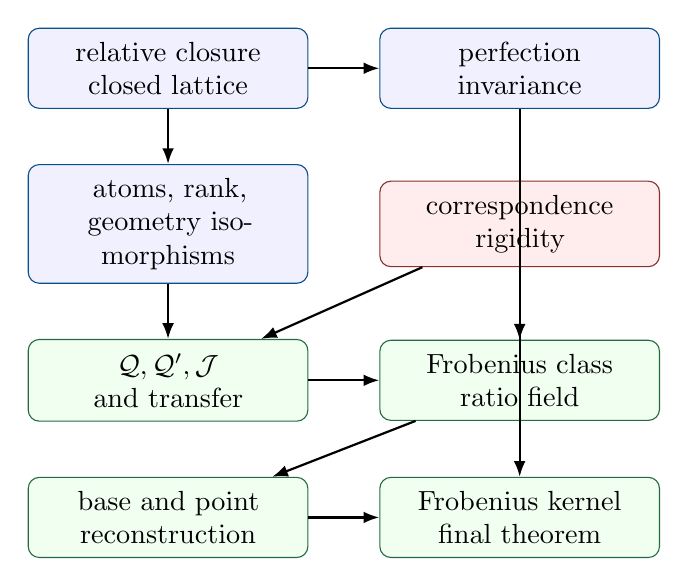
\begin{tikzpicture}[
  node distance=7mm and 9mm,
  box/.style={draw,rounded corners,align=center,inner sep=5pt,text width=32mm},
  hard/.style={box,fill=red!7,draw=brick},
  base/.style={box,fill=blue!6,draw=leanblue},
  glue/.style={box,fill=green!6,draw=darkgreen},
  arr/.style={-{Latex[length=2mm]},thick}
]
\node[base] (acl) {relative closure\\closed lattice};
\node[base,right=of acl] (perf) {perfection\\invariance};
\node[base,below=of acl] (geom) {atoms, rank,\\geometry isomorphisms};
\node[hard,right=of geom] (rigid) {correspondence\\rigidity};
\node[glue,below=of geom] (config) {$\Qrel,\Qprel,\Jrel$\\and transfer};
\node[glue,right=of config] (interp) {Frobenius class\\ratio field};
\node[glue,below=of config] (recon) {base and point\\reconstruction};
\node[glue,right=of recon] (kernel) {Frobenius kernel\\final theorem};
\draw[arr] (acl)--(geom);
\draw[arr] (acl)--(perf);
\draw[arr] (geom)--(config);
\draw[arr] (rigid)--(config);
\draw[arr] (config)--(interp);
\draw[arr] (perf)--(interp);
\draw[arr] (interp)--(recon);
\draw[arr] (recon)--(kernel);
\draw[arr] (rigid)--(kernel);
\end{tikzpicture}
\end{center}

There should be no circular dependency between the semantic field relations and their
geometric definitions.  Put semantic relations in a file that imports only field and
closure foundations; put geometric predicates in a separate file; prove equivalence in a
third file.  The interpreted field may use semantic decoding to obtain its field instance,
but its naturality theorem must be proved solely from geometric characterizations.

\section{Foundation I: relative closure as a pregeometry}

Fix fields $k,K$ with an algebra structure $k\to K$.  For $S\subseteq K$, define
\[
  \operatorname{racl}_{k}^{K}(S)
  =\{x\in K:x\text{ is algebraic over }k(S)\}.
\]
In Lean, first form \lean{IntermediateField.adjoin k S}, take
\lean{algebraicClosure} of its underlying field in $K$, and restrict scalars back to $k$.
Expose a carrier-level membership theorem immediately; subsequent proofs should almost
never unfold the tower of intermediate-field definitions.

The Lean definition is the restriction of
{\small\lean{algebraicClosure (IntermediateField.adjoin k S) K}} along the evident scalar
tower.  Its public membership theorem is
\[
 x\in\operatorname{racl}_{k}^{K}(S)
 \quad\Longleftrightarrow\quad
 \text{$x$ is algebraic over the fraction field generated by $k\cup S$}.
\]
No later proof unfolds the restriction-of-scalars implementation.

\begin{proposition}[relative algebraic closure is a pregeometry]
The operator $\operatorname{racl}_{k}^{K}$ is extensive, monotone, idempotent, has
finite character, and satisfies exchange.  It is equivariant under isomorphisms of field
extensions.  If $K$ is perfect of characteristic exponent $p$, it is invariant under
every integral Frobenius iterate.
\end{proposition}
\begin{proof}
Put $F_S=k(S)\subseteq K$.

Extensivity holds because each $s\in S$ already belongs to $F_S$.  If $S\subseteq T$,
then $F_S\subseteq F_T$, and a polynomial over $F_S$ witnessing algebraicity is also a
polynomial over $F_T$; this proves monotonicity.

For idempotence, let $x$ be algebraic over
$F_{\operatorname{racl}(S)}$.  A monic polynomial for $x$ uses only finitely many
coefficients, and every coefficient is a rational expression in finitely many elements
$z_1,\ldots,z_m$ of $\operatorname{racl}(S)$.  Each $z_i$ is algebraic over $F_S$.
Consequently $F_S(z_1,\ldots,z_m)/F_S$ is finite, while $x$ is algebraic over that
finite extension.  Transitivity of algebraicity gives that $x$ is algebraic over $F_S$.
The reverse inclusion follows from extensivity.

The same finiteness argument proves finite character more directly.  If
$f(X)\in F_S[X]$ is a nonzero polynomial with $f(x)=0$, every coefficient of $f$ is a
quotient of two polynomials involving only finitely many members of $S$.  The union $T$
of these finite supports is finite, $T\subseteq S$, and $f\in F_T[X]$, so
$x\in\operatorname{racl}(T)$.

For exchange, set $F=F_S$ and suppose
$x\in\acl_F(y)\setminus\acl_F(\varnothing)$.  Thus $x$ is transcendental over $F$ and
algebraic over $F(y)$.  If $y$ were transcendental over $F(x)$, then $(x,y)$ would be
algebraically independent over $F$ and $\trdeg_FF(x,y)=2$.  On the other hand,
algebraicity of $x$ over $F(y)$ gives
$\trdeg_FF(x,y)=\trdeg_FF(y)\leq1$, a contradiction.  Hence $y$ is algebraic over
$F(x)$, which is exactly
$y\in\operatorname{racl}(S\cup\{x\})$.

Let $\sigma:K\simeq L$ carry $k$ onto $l$.  It carries $F_S$ onto
$l(\sigma S)$, transports a nonzero annihilating polynomial coefficient by coefficient,
and the same argument with $\sigma^{-1}$ gives
\[
 \sigma(\operatorname{racl}_{k}^{K}(S))
   =\operatorname{racl}_{l}^{L}(\sigma S).
\]
Finally, on a perfect field Frobenius is an automorphism fixing the prime field.  For
$q=p^n$ with $n\geq0$, each $s$ is algebraic (indeed purely inseparable) over $s^q$
and conversely $s^q\in k(s)$.  Therefore $F_S$ and $F_{S^q}$ have the same algebraic
closure in $K$.  Applying the same statement to inverse Frobenius handles $n<0$.
All uses of finite extensions, transitivity of algebraicity, transcendence degree in an
algebraic tower, and Frobenius equivalences are supplied by Mathlib; the argument above
is the project-local glue.
\end{proof}

\begin{lemma}[finite representative calculus]\label{lem:finite-representative-calculus}
Let $v_1,\ldots,v_n\in K$.
\begin{enumerate}[label=(\alph*),leftmargin=10mm]
\item The tuple is algebraically independent over $k$ if and only if, for every $i$,
$v_i\notin\operatorname{racl}_k(\{v_j:j\neq i\})$.
\item Replacing every $v_i$ by $w_i$ with
$\operatorname{racl}_k(v_i)=\operatorname{racl}_k(w_i)$ preserves algebraic
independence and every finite rank.
\item If $\trdeg_kK\geq5$ and a finite tuple $c$ has rank $r<5$, there is
$t\notin\acl_k(c)$.  If $r<4$, there are successive $s,t$ such that $(c,s,t)$ has
rank $r+2$.
\item Any birational monomial or affine change of coordinates preserves independence
on its domain.  In particular the changes
$(x,y,a)\mapsto(xa,ya,a)$,
$(x,y,a)\mapsto(x(1+a),y(1+a),a)$, and
$(x,y,a)\mapsto(xy,y,a)$ preserve the ranks used below whenever the displayed
denominators are nonzero.
\end{enumerate}
\end{lemma}
\begin{proof}
For (a), dependence gives a nonzero polynomial in the $v_i$.  Regard it as a polynomial
in a variable which occurs with positive degree; that $v_i$ is algebraic over the other
entries.  The converse is immediate from an annihilating polynomial.  Part (b) follows
by replacing entries one at a time and applying exchange: adjoining interalgebraic
elements gives algebraic field extensions in both directions and hence does not alter
transcendence degree.  For (c), extend a maximal independent subtuple of $c$ to a
transcendence basis of $K/k$; the next one or two basis elements are the required fresh
elements.  For (d), write the rational inverse explicitly---for example
$x=(xa)/a$, $y=(ya)/a$, and $a=a$---and use invariance of transcendence degree under
an isomorphism of rational function fields.  The other listed maps have inverses obtained
by division by $1+a$ or by $y$.
\end{proof}

\section{Foundation II: the complete atomistic lattice}

\begin{definition}
For an intermediate field $E$ of $K/k$, put
\[
  \operatorname{IsRAC}(E):\Longleftrightarrow
  \operatorname{algebraicClosure}_{K}(E)=E,
\]
represented in Mathlib's tower convention by
\lean{algebraicClosure (Subtype E) K = bot}.  Define
\[
  \operatorname{ClosedIF}(k,K)=\{E:\operatorname{IntermediateField}(k,K)\mid
  \operatorname{IsRAC}(E)\}.
\]
\end{definition}

Under the theorem hypothesis \lean{algebraicClosure k K = bot}, the bottom member is
the image of $k$ and the top member is $K$.

\subsection{Complete-lattice construction}

Order by inclusion.  The infimum of a family is the ordinary intersection of its
carriers, and define the supremum by
\[
  \bigvee_{\G} E_i=\RAC_K\!\left(\bigvee_{\operatorname{IntermediateField}}E_i\right).
\]

\begin{proposition}[complete lattice]\label{prop:closed-complete-lattice}
These operations make $\G(K/k)$ a complete lattice.  Its bottom is $k$, its top is $K$,
and a base-preserving field equivalence induces an order isomorphism of these lattices.
\end{proposition}
\begin{proof}
Let $E=\bigcap_iE_i$ and let $x\in K$ be algebraic over $E$.  The same annihilating
polynomial has coefficients in every $E_i$, so $x$ is algebraic over every $E_i$.
Relative algebraic closedness gives $x\in E_i$ for every $i$, hence $x\in E$; thus $E$
is closed.  This intersection plainly has the greatest-lower-bound property.

For the supremum, put $F=\RAC_K(\langle\bigcup_iE_i\rangle)$.  Extensivity gives
$E_i\subseteq F$.  If a relatively algebraically closed $N$ contains every $E_i$, it
contains their compositum.  Every element of $F$ is algebraic over that compositum and
hence algebraic over $N$; closedness of $N$ puts it in $N$.  Therefore $F$ is the least
upper bound.  The empty intersection is $K$.  The empty compositum is $k$, and the
hypothesis that $k$ is relatively algebraically closed identifies its relative closure
with $k$.

If $\sigma:(K/k)\simeq(L/l)$ is a field-extension isomorphism, equivariance of relative
closure shows that $E\mapsto\sigma(E)$ and $F\mapsto\sigma^{-1}(F)$ preserve closed
members and are inverse monotone maps.  This is the required order isomorphism.  In Lean,
extensionality of intermediate fields supplies all equality goals; arbitrary infima use
carrier intersection and arbitrary suprema use the membership theorem for relative
closure.
\end{proof}

\subsection{Atoms and principal closures}

For $x\notin k$, let $P_x=\operatorname{racl}_k^K(\{x\})$ as a closed intermediate
field.  Relative algebraic closedness of $k$ implies that $x$ is transcendental over $k$.
Use exchange to prove:

\begin{lemma}[principal closures are atoms]\label{lem:principal-atom}
$P_x$ is an atom of $\G(K/k)$.  Conversely, every atom is $P_x$ for some $x\notin k$.
Moreover $P_x=P_y$ iff $x$ and $y$ are interalgebraic over $k$.
\end{lemma}
\begin{proof}
For the forward direction, if $\bot<F\leq P_x$, choose $y\in F\setminus k$.
Then $y\in\acl_k(x)\setminus\acl_k(\varnothing)$, so exchange gives
$x\in\acl_k(y)$.  Since $F$ is relatively algebraically closed, $x\in F$, hence
$P_x\leq F$.  For the converse, choose $x$ in a non-bottom atom $P$; then
$\bot<P_x\leq P$, so atomicity gives equality.
Finally $P_x=P_y$ implies $x\in\acl_k(y)$ and $y\in\acl_k(x)$ by extensivity; the
reverse implication follows from monotonicity and idempotence in both directions.
\end{proof}

\begin{lemma}[atomisticity]\label{lem:atomistic}
For every $E\in\G(K/k)$,
\[
  E=\bigvee\{P:P\text{ is an atom and }P\leq E\}.
\]
\end{lemma}
\begin{proof}
The join on the right is at most $E$.  Conversely, every $x\in E\setminus k$ lies in
the atom $P_x\leq E$, while elements of $k$ lie in the bottom and therefore in every
closed intermediate field.  Thus the two carriers are equal.
\end{proof}

\subsection{Point geometry and equivalence of presentations}

Define
\[
  \operatorname{Point}(k,K)=\{P\in\G(K/k):P\text{ is an atom}\}
\]
and, for $S\subseteq\operatorname{Point}(k,K)$,
\[
  \operatorname{pointCl}(S)=\{P:P\leq\bigvee_{Q\in S}Q\}.
\]
The pregeometry axioms follow as follows.  Extensivity and monotonicity are immediate from
the order.  For idempotence,
$P\leq\bigvee\{Q:Q\leq\bigvee S\}$ if and only if $P\leq\bigvee S$, because the latter
join is itself an upper bound of all the displayed $Q$.  Finite character follows from
finite character of relative algebraic closure after choosing representatives of the
finitely many coefficients.  For exchange, write $P=P_x$, $Q=P_y$, choose
representatives for the atoms in $S$, and apply exchange for
$\operatorname{racl}$; \cref{lem:principal-atom} converts the result back to atoms.

The two comparison maps are
\[
  E\longmapsto\{P:P\leq E\},\qquad
  S\longmapsto\bigvee S.
\]
On a closed point set $S$, the first composite is
$\{P:P\leq\bigvee S\}=\operatorname{pointCl}(S)=S$; on $E\in\G(K/k)$, the second
composite is $\bigvee\{P:P\leq E\}=E$ by atomisticity.  Thus the two maps are inverse
order isomorphisms.

An order isomorphism carries bottom to bottom and atoms to atoms: the definition of atom
uses only strict inequalities above bottom.  It preserves arbitrary suprema and infima
because an element is the supremum of a family exactly when it satisfies the order-theoretic
least-upper-bound predicate, and similarly for infima.  It consequently preserves point
closure.  Conversely, a closure-preserving point equivalence sends closed point sets to
closed point sets and its inverse does the same, so direct image gives an order isomorphism.
The two constructions are inverse by the preceding composite calculations.  Finally,
finite independence is the assertion that no point lies in the closure of its predecessors;
hence it and the maximum length of an independent tuple below a closed element are
preserved.  This proves every point/lattice transport fact used later without cardinal
arithmetic.

For the first implementation, define finite rank geometrically.  For a closed lattice
element $E$, say \lean{RankLE n E} if $E$ is below the join of $n$ atoms; say
\lean{RankEq n E} if it is generated by an independent $n$-tuple of atoms.  Prove agreement
with $\operatorname{trdeg}$ only after the configuration API is stable.  This avoids a
premature dependency on cardinal arithmetic.

\section{Foundation III: invariance under perfection}

Let $\iota:K\to K^{\mathrm{perf}}$ be a chosen perfect closure with exponent $p$, and
let $M\in\G(K/k)$.  Define
\[
 M^{\mathrm{perf}}
 =\{x\in K^{\mathrm{perf}}:\exists n,\ x^{p^n}\in\iota(M)\}.
\]
Use Mathlib's relative \lean{perfectClosure} to obtain the subfield structure, but expose
the displayed membership theorem as the public API.

\begin{proposition}[perfection order isomorphism]\label{prop:perf-lattice}
The assignment $M\mapsto M^{\mathrm{perf}}$ is an order isomorphism
\[
  \G(K/k)\simeq_o\G(K^{\mathrm{perf}}/k^{\mathrm{perf}}),
\]
whose inverse is intersection with $K$ (implemented as comap along $\iota$).
It preserves atoms and the point closure operation.
\end{proposition}
\begin{proof}
We give the positive-characteristic proof; when the characteristic exponent is $1$ all
perfect closures and all powers below are the original objects.

First $k^{\mathrm{perf}}$ is relatively algebraically closed in
$K^{\mathrm{perf}}$.  Let $x\in K^{\mathrm{perf}}$ be algebraic over
$k^{\mathrm{perf}}$.  Choose $r$ with $x^{p^r}\in K$.  A finite set of coefficients
of an annihilating polynomial for $x$ has a common $p^s$-power in $k$.  Raising the
polynomial identity to the $p^s$th power shows that $x^{p^s}$, and therefore
$x^{p^{r+s}}$, is algebraic over $k$.  Since the latter element lies in $K$ and $k$ is
relatively algebraically closed in $K$, it lies in $k$.  The membership criterion for a
perfect closure now gives $x\in k^{\mathrm{perf}}$.  Replacing $k$ by any closed $M$
proves that $M^{\mathrm{perf}}$ is closed in $K^{\mathrm{perf}}$.

If $x\in K\cap M^{\mathrm{perf}}$, then $x^{p^r}\in M$ for some $r$.  Thus $x$ is
algebraic over $M$, and closedness of $M$ gives $x\in M$.  The other inclusion is
immediate, so
\[
 K\cap M^{\mathrm{perf}}=M.                                      \tag{5.1}
\]
Conversely let $N$ be closed between $k^{\mathrm{perf}}$ and
$K^{\mathrm{perf}}$.  For $x\in N$, choose $r$ with $x^{p^r}\in K$.  Since $N$ is a
field, $x^{p^r}\in N\cap K$, whence $x\in(N\cap K)^{\mathrm{perf}}$.  For the reverse
inclusion, first observe that $N$ is perfect.  If $z\in N$ and $y^p=z$ in
$K^{\mathrm{perf}}$, then $y$ is algebraic over $N$; relative algebraic closedness of
$N$ puts $y$ in $N$.  Iterating gives closure under every $p^r$th root.  Therefore
$y^{p^r}\in N\cap K$ implies $y\in N$, and hence
\[
 (N\cap K)^{\mathrm{perf}}=N.                                   \tag{5.2}
\]
Equations (5.1) and (5.2) show that perfection and intersection are inverse order maps.

For naturality, if $\sigma:K^{\mathrm{perf}}\simeq L^{\mathrm{perf}}$ is a field
equivalence, then
$x^{p^r}\in M$ if and only if $\sigma(x)^{p^r}=\sigma(x^{p^r})\in\sigma(M)$.
Thus $\sigma(M^{\mathrm{perf}})=\sigma(M)^{\mathrm{perf}}$ by extensionality.
Order isomorphisms preserve atoms and joins, so the point geometry is preserved.
Finally $x$ and $x^{p^r}$ are interalgebraic, and inverse Frobenius handles negative
$r$; therefore every integral Frobenius iterate fixes every atom.
\end{proof}

After \cref{prop:perf-lattice}, the reconstruction proof may assume without loss of
generality that the ambient fields are perfect and the bases relatively algebraically
closed.  The final theorem transports the result back through these order isomorphisms.

\section{A small geometry language for finite configurations}

Do not begin by encoding the countable first-order language
$\{\acl_n:n\in\mathbb N\}$.  The proof only uses a fixed finite collection of relations,
and Lean propositions are easier to transport through a geometry isomorphism.

For points $P,Q,R$, define
\[
\begin{aligned}
  P\in\cl(Q_1,\ldots,Q_n)&:\Longleftrightarrow
       P\leq Q_1\vee\cdots\vee Q_n,\\
  \operatorname{Col}(P,Q,R)&:\Longleftrightarrow
       R\leq P\vee Q,\\
  \operatorname{Line}(P,Q)&=P\vee Q.
\end{aligned}
\]
Whenever collinearity is intended to describe a genuine line, include $P\neq Q$ and
the required distinctness hypotheses.  For closed elements use joins and meets directly.

\begin{definition}[partial quadrangle]\label{def:partialquad}
Six distinct points $(S,T,U,S',T',U')$ form a partial quadrangle if the four triples
\[
 (S,T,U),\quad(S,T',U'),\quad(S',T,U'),\quad(S',T',U)
\]
have rank two, every other three-element subtuple has rank three, and the join of all six
has rank three.  Implement the ``every other'' clause by quantifying over
three-element finsets of \lean{Fin 6}; prove a finite simplification lemma giving the four
named dependent triples.
\end{definition}

This is the orientation used in the Evans--Hrushovski group configuration.  If the
published figure is transcribed with a different ordering, prove one permutation lemma
and keep a single canonical Lean definition.

For any geometry equivalence $f$, prove one generic recursion theorem saying that formulas
built from equality, point-below-join, equality of finite joins/meets, Boolean operations,
and point quantifiers are invariant under $f$.  The concrete predicates below can then be
proved invariant with short \lean{simpa} arguments.

\section[The semantic relations Q, Q-prime, and J]
{The semantic relations $\Qrel$, $\Qprel$, and $\Jrel$}

Work now in a perfect relatively algebraically closed extension $K/k$.  If $x\notin k$,
write $[x]$ for the atom $\acl_k(x)$.

\begin{definition}[semantic configurations]\label{def:semantic-configs}
For points $X,Y,Z,W$, define
\[
\begin{aligned}
\Qrel_{\rm sem}(X,Y,Z,W)
&\Longleftrightarrow
 \exists x,y\text{ algebraically independent over }k,\\[-2mm]
&\hspace{18mm}(X,Y,Z,W)=([x],[y],[x+y],[x/y]);\\
\Qprel_{\rm sem}(X,Y,Z,W)
&\Longleftrightarrow
 \exists x,y\text{ algebraically independent over }k,\\[-2mm]
&\hspace{18mm}(X,Y,Z,W)=([x],[y],[x+y],[xy]).
\end{aligned}
\]
For independent $x,a$, put
\[
 j(x,a)=([x],[x+a],[xa],[x+xa],[a])
\]
and let $\Jrel_{\rm sem}$ be the image of $j$.
\end{definition}

The normalization identities used below require no extra theorem.  If $0\neq c\in k$,
then $x=c^{-1}(cx)$ and $cx\in k(x)$, so $[cx]=[x]$; similarly
$x=(x+c)-c$ gives $[x+c]=[x]$.  An element and any positive Frobenius power are
purely inseparably interalgebraic, and inverse Frobenius handles negative powers in a
perfect field.  Applying these observations coordinatewise proves all tuple versions.

\section[The geometric definition of Q]
{The geometric definition of $\Qrel$}\label{sec:psi}

Gismatullin makes the Evans--Hrushovski witness completely explicit.  The following is a
direct lattice translation.  All displayed capital letters denote points; juxtaposition
inside $\cl$ means join.

Given
\[
(A_1,A_2,B_1,B_2,C_1,C_2,D,E,F,G,H,I,P,Q,R,S,T,U,X,Y,Z),
\]
put $A=A_1\vee A_2$, $B=B_1\vee B_2$, and $C=C_1\vee C_2$.
Define $\Psi$ to be the conjunction of:

\begin{enumerate}[label=(\roman*),leftmargin=12mm]
\item
$\rk(A\vee B\vee C)=\rk(A\vee B)=\rk(B\vee C)=\rk(A\vee C)=4$;
\item $X\leq A\vee Y$ and
$Z\leq(B\vee Y)\wedge(C\vee X)$;
\item $X,Y,Z\not\leq A\vee B\vee C$;
\item for every atom $A'\leq A$, $X\not\leq A'\vee Y$;
for every atom $B'\leq B$, $Z\not\leq B'\vee Y$; and for every atom
$C'\leq C$, $Z\not\leq C'\vee X$;
\item $S\leq A$, $T\leq B$, $U\leq C$, and $\rk(S\vee T\vee U)=2$;
\item there exist $S',T',U'$ such that
$(S,T,U,S',T',U')$ is a partial quadrangle in the sense of
\cref{def:partialquad};
\item the seven intersection equations
\[
\begin{aligned}
(P\vee Y)\wedge(S\vee X)&=D,&
(T\vee Y)\wedge(Q\vee Z)&=E,\\
(U\vee X)\wedge(T\vee D)&=F,&
(P\vee T)\wedge(Q\vee R)&=G,\\
(H\vee X)\wedge(P\vee Y)&=I,&
(U\vee G)\wedge A&=H,\\
(F\vee Z)\wedge C&=R.&
\end{aligned}
\]
\end{enumerate}

Then define
\[
 \Qrel_{\rm geom}(P,D,Y,I)
 \Longleftrightarrow
 \exists A_1,A_2,B_1,B_2,C_1,C_2,E,F,G,H,Q,R,S,T,U,X,Z\;\Psi.
\]
(The quantified $S',T',U'$ live inside clause (vi).)  In Lean, use a structure
\lean{QWitness} with named fields rather than a 21-tuple; this makes the intersection
equations readable and prevents permutation errors.

The central correctness result is:

\begin{theorem}[configuration correctness for $\Qrel$]\label{thm:q-correct}
In an algebraically closed extension of algebraically closed fields of transcendence degree
at least five,
\[
  \Qrel_{\rm geom}=\Qrel_{\rm sem}.
\]
\end{theorem}
\begin{proof}
We first work over algebraically closed $k\subseteq K$.

For soundness, suppose the semantic tuple is
$([u],[v],[u+v],[u/v])$ with $u,v$ independent.  Choose $a$ transcendental over
$k(u,v)$, put $b=u$ and $x=v/a$, and choose successive $c,d$ algebraically independent
over $k(a,b,x)$.  Then $a,b,c,d,x$ are independent and $ax=v$.  Use the following
complete witness table (entries denote their rank-one closures):
\[
\begin{array}{c|ccccccccccc}
 &A_1&A_2&B_1&B_2&C_1&C_2&P&Q&R&S&T\\ \midrule
 &a&b&c&d&ac&bc+d&b&d&bc+d&a&c\\[1mm]
\hline
 &U&X&Y&Z&D&E&F&G&H&I\\ \midrule
 &ac&x&ax+b&c(ax+b)+d&ax&c(ax+b)&acx&bc&a/b&ax/b
\end{array}                                                     \tag{7.1}
\]
For the partial quadrangle take
\[
 S'=b,\qquad T'=acb,\qquad U'=cb.                              \tag{7.2}
\]

We verify every clause.  The rational changes
\[
 (a,b,c,d)\longleftrightarrow(a,b,ac,bc+d),\qquad
 (a,b,c,d)\longleftrightarrow(c,d,ac,bc+d)
\]
have the displayed inverses $c=(ac)/a$, $d=(bc+d)-bc$ and
$a=(ac)/c$, $b=((bc+d)-d)/c$.  Hence every pair among $A,B,C$ and their total join has
rank four, proving (i).  The formulas
\[
 x=(Y-b)/a,\qquad Z=cY+d=(ac)x+(bc+d)
\]
prove (ii).  Since $x$ is transcendental over $k(a,b,c,d)$, each of $X,Y,Z$ is outside
$A\vee B\vee C$, proving (iii).

For clause (iv) we record the elementary minimal-parameter calculation.  Suppose
$t\in\acl(a,b)$ has rank one and $x\in\acl(t,ax+b)$.  The intersection
$\acl_k(t)\cap k(a,b)$ has transcendence degree one; choose in it a separating
transcendence generator and rename it $t$.  This replacement is interalgebraic with the
old $t$, does not change its point, puts $t$ in $k(a,b)$, and ensures that its
differential in $k(a,b)/k$ is nonzero.  Put $Y=ax+b$.  The field
$F=k(t,x,Y)$ has transcendence degree two: $t,x$ are independent, while the supposition
makes $x$ algebraic over $k(t,Y)$.  The field $E=k(a,b,x)$ has transcendence degree
three, so a separating transcendence basis for the finitely generated extension $E/F$
supplies a nonzero $F$-derivation $D:E\to E'$ into a finite algebraic overfield.  It
satisfies
\[
 0=D(ax+b)=xD(a)+D(b),\qquad
 0=D(t)=(t_a-xt_b)D(a).
\]
Here $t_a,t_b$ are the coefficients of $dt=t_a,da+t_b,db$ after the finite separable
replacement; they are not both zero.  Substitution of $D(b)=-xD(a)$ gives
$(t_a-xt_b)D(a)=0$.  Independence of $x$ from $a,b$ makes the coefficient nonzero.
Thus $D(a)=D(b)=D(x)=0$, contradicting the choice of a nonzero $F$-derivation on the
field generated by $a,b,x$.  Therefore
$x\notin\acl(t,Y)$.  Applying the same calculation after the birational substitutions
$(a,b,x)\mapsto(c,d,Y)$ and $(c,d,Y)\mapsto(ac,bc+d,x)$ proves the two assertions for
$B'$ and $C'$.

The monomial exponent vectors of $(S,T,U,S',T',U')$ with respect to the independent
triple $(a,c,b)$ are
\[
 (1,0,0),(0,1,0),(1,1,0),(0,0,1),(1,1,1),(0,1,1).
\]
The four named triples have rank two because respectively
$U=ST$, $T'=SU'$, $U'=S'T$, and $T'=S'U$.  For reference, the nonexceptional
determinants are $+1$ for
\[
 STS',\ STT',\ STU',\ SUS',\ SUT',\ SUU',\ TS'T',\ S'T'U'
\]
and $-1$ for
\[
 SS'T',\ SS'U',\ TUS',\ TUT',\ TUU',\ TT'U',\ US'U',\ UT'U'.
\]
These are all sixteen remaining triples, so each has rank three; the total rank is three.
This proves (v)--(vi).  Finally each of the seven meets is the corresponding row of the
independent-variable intersection calculation in the proof of
\cref{lem:affine-grid-extraction}; it gives exactly $D,E,F,G,H,I,R$ in (7.1).  Thus
$\Psi$ holds.  Its four free outputs are
\[
 (P,D,Y,I)=([b],[ax],[b+ax],[ax/b])
          =([u],[v],[u+v],[u/v]),
\]
because a nonzero element and its inverse generate the same rank-one closure.

For completeness, suppose $\Psi$ holds.  Apply
\cref{lem:affine-grid-extraction}.  It supplies independent $a,b,c,d,x$ and identifies
\[
 (P,D,Y,I)=([b],[ax],[b+ax],[ax/b]).
\]
The pair $(b,ax)$ is independent: adjoining it to $a$ is birationally equivalent to
adjoining $(a,b,x)$.  Its sum is $b+ax$, and its ratio $b/(ax)$ has the same closure as
$ax/b$.  Hence the displayed tuple belongs to $\Qrel_{\rm sem}$.

\end{proof}

\section[The multiplication diagram and Q-prime]
{The multiplication diagram and $\Qprel$}

The projective multiplication diagram can be stated without a picture.  Take eight
pairwise distinct points
\[
  X,Y,V,E,A_0,B_0,C_0,D_0.
\]
Define
\lean{MulDiagram X Y V E A0 B0 C0 D0} by the following rank-two lines:
\[
\begin{array}{llll}
\{X,A_0,B_0\}, & \{A_0,Y,C_0\}, & \{A_0,E,D_0\},&
\{B_0,Y,D_0\},\\
\{X,C_0,D_0\},& \{B_0,C_0,V\},&
\{X,Y,E,V\}.&
\end{array}
\]
The last entry means that all four points lie on the same rank-two line.  Require also
$\rk(X\vee Y\vee A_0)=3$ and that every displayed line is genuine (any two named points
on it are distinct).  These nondegeneracy clauses rule out collapsed diagrams.

\begin{lemma}[coordinate check for the multiplication diagram]\label{lem:mul-diagram}
If $x,y,a$ are algebraically independent, the assignment
\[
\begin{array}{c|cccccccc}
\text{point}&X&Y&V&E&A_0&B_0&C_0&D_0\\ \midrule
\text{representative}&x&y&x/y&xy&a&ax&ay&axy
\end{array}
\]
satisfies \lean{MulDiagram}.  Conversely, a nondegenerate diagram with bottom points
$[x],[y],[x/y]$ has $E=[xy]$ and admits representatives of the displayed form, up to
the correspondence ambiguity controlled by \cref{sec:rigidity}.
\end{lemma}
\begin{proof}
For the displayed representatives, every line follows from one rational identity:
$ax=a\cdot x$, $ay=a\cdot y$, $axy=a\cdot xy=(ax)y=x(ay)$, and
$(ax)/(ay)=x/y$.  Each two named points on a line are independent and
$(x,y,a)$ has rank three, so all nondegeneracy clauses hold.

Conversely choose independent representatives $x,y,a$ for $X,Y,A_0$; the rank-three
condition permits this by \cref{lem:finite-representative-calculus}.  Every rank-two line
in the diagram is an irreducible three-way finite correspondence: for example a generic
representative of $B_0$ is algebraic over $(x,a)$ and each of $x,a$ is algebraic over the
other one together with it.  Compose the correspondences around the four triangles
\[
 (X,A_0,B_0),\quad(A_0,Y,C_0),\quad(B_0,C_0,V),
 \quad(X,Y,V).
\]
The two paths from $(x,a,y)$ to $V$ agree.  Applying
\cref{lem:curve-coset} to their independent generic fibers produces a common
one-dimensional group.  The last triangle is already the multiplicative relation
$V=[x/y]$; hence \cref{lem:subgroup-classification}(b) identifies that group with
$\Gm$ and gives monomial coordinates on every side.  Raise representatives to common
nonzero powers and absorb base scalars.  These operations do not change their rank-one
closures, and the four triangles then read literally
\[
 B_0=[ax],\qquad C_0=[ay],\qquad V=[x/y].                       \tag{7.3}
\]
The triangles $(B_0,Y,D_0)$ and $(X,C_0,D_0)$ now give two generic products with the
same output.  The multiplicative correspondence theorem forces
$D_0=[axy]$; a different exponent would contradict the already synchronized $x$- and
$y$-edges in (7.3).  Finally $(A_0,E,D_0)$ gives
$E=[D_0/a]=[xy]$.  This also proves that the normalized representatives have exactly the
form in the table.  All normalization steps are finite algebraic covers, so equality of
points, which is equality of algebraic closures, is unaffected.
\end{proof}

Define
\[
\begin{split}
\Qprel_{\rm geom}(X,Y,S,E)\Longleftrightarrow
\exists V,A_0,B_0,C_0,D_0,\;&\Qrel_{\rm geom}(X,Y,S,V)\\
&\land\operatorname{MulDiagram}(X,Y,V,E,A_0,B_0,C_0,D_0).
\end{split}
\]
\begin{theorem}[configuration correctness for $\Qprel$]\label{thm:qp-correct}
Over algebraically closed fields of relative transcendence degree at least five,
$\Qprel_{\rm geom}=\Qprel_{\rm sem}$.
\end{theorem}
\begin{proof}
If $\Qprel_{\rm geom}(X,Y,S,E)$ holds, \cref{thm:q-correct} supplies independent
$x,y$ with
$(X,Y,S,V)=([x],[y],[x+y],[x/y])$.  The converse half of
\cref{lem:mul-diagram} then gives $E=[xy]$, so the tuple is semantic.

Conversely start with $([x],[y],[x+y],[xy])$ for independent $x,y$.  Put
$V=[x/y]$, so \cref{thm:q-correct} gives the required $\Qrel$ witness.  Choose
$a$ transcendental over $k(x,y)$ and take
$A_0=[a],B_0=[ax],C_0=[ay],D_0=[axy]$.  The forward half of
\cref{lem:mul-diagram} supplies the second conjunct.  This proves equality of the two
relations.
\end{proof}

The definition is invariant under every geometry isomorphism because it uses only rank,
equality, joins, meets, incidence, and point quantifiers, all of which an order isomorphism
preserves.

\section[The geometric definition of J]
{The geometric definition of $\Jrel$}

Evans--Hrushovski's identity, reproduced by Gismatullin, is
\[
\begin{split}
\Jrel_{\rm geom}(X,P,Q,R,A)\Longleftrightarrow{}&
\Qrel_{\rm geom}(X,Q,R,A)\\
&\land\Qprel_{\rm geom}(X,A,P,Q)\\
&\land\Qprel_{\rm geom}(X,A,P,R).
\end{split}
\]
The last occurrence is correct: it uses $[a+1]=[a]$ and
$x(a+1)=x+xa$.

\begin{theorem}[correctness of $\Jrel$ over algebraically closed fields]
\label{thm:j-acf-correct}
\[
  \Jrel_{\rm geom}=\Jrel_{\rm sem}
\]
over algebraically closed $k\subseteq K$ of relative transcendence degree at least five.
\end{theorem}
\begin{proof}
If $(X,P,Q,R,A)=j(x,a)$, then
\[
 (X,Q,R,A)=([x],[xa],[x+xa],[x/(xa)])
\]
belongs to $\Qrel$, because $[1/a]=[a]$.  The tuple
$(X,A,P,Q)=([x],[a],[x+a],[xa])$ belongs to $\Qprel$.  For the last conjunct use
$a+1$ as representative of $A$: then
\[
 ([x],[a+1],[x+(a+1)],[x(a+1)])=(X,A,P,R),
\]
because adding the base element $1$ does not change $P$.

Conversely assume the three semantic conjuncts.  From the first $\Qprel$ conjunct choose
independent $x,a$ so that
\[
 (X,A,P,Q)=([x],[a],[x+a],[xa]).                               \tag{7.4}
\]
Choose representatives for the other two conjuncts.  Equality of their $X$- and
$A$-points with those in (7.4) gives two finite correspondence curves.  Equality of the
two $P$-points supplies the coordinatewise additive relation, while equality of $Q$ and
the quotient coordinate in the $\Qrel$ conjunct supplies the coordinatewise
multiplicative relation.  Hence the two curves are simultaneous additive and
multiplicative cosets.  By \cref{lem:simultaneous-coset} all representatives differ from
$x,a$ by one common Frobenius power and one common scalar.  The last $\Qprel$ conjunct
uses both $a$ and $a+1$; exactly the coefficient comparison in the proof of
\cref{thm:jrigidity} forces that scalar to be $1$.  Frobenius does not change a point.
Consequently the remaining coordinate is
\[
 R=[x(a+1)]=[x+xa],
\]
and the whole tuple is $j(x,a)$.  This proves the reverse implication.
\end{proof}

Over arbitrary perfect relatively algebraically closed fields the same equality is
proved, without an ACF black box, in \cref{thm:j-descent}.  The useful projection
\[
 \Qrel(X,Q,R,A)\Longleftrightarrow\exists P\;\Jrel(X,P,Q,R,A)
\]
follows semantically: from a $\Qrel$ witness in the form
$([x],[xa],[x+xa],[a])$ take $P=[x+a]$, and the reverse implication is the first conjunct
of the definition.  Transport through the correctness theorems gives the geometric
version.  The corresponding $\Qprel$ projections are identical coordinate eliminations.

\section{The hard kernel: algebraic-correspondence rigidity}\label{sec:rigidity}

This section proves, rather than imports, the fragment of geometric stability theory used
by Evans--Hrushovski.  Throughout it, $k\subseteq\Omega$ are algebraically closed fields
and all algebraic closures are taken in $\Omega$.  For a tuple $a$, let
\[
 I(a/k)=\{f\in k[X_1,\ldots,X_n]:f(a)=0\},\qquad
 \Loc_k(a)=V(I(a/k)).
\]
The ideal $I(a/k)$ is prime because evaluation maps the polynomial ring into the field
$\Omega$; hence $\Loc_k(a)$ is irreducible.  Its function field is the fraction field of
$k[a]$, and its dimension is $\trdeg_k k(a)$.  Thus every occurrence of ``generic'' below
means only that the displayed tuple has the stated transcendence degree.

\subsection{Finite correspondences and rational group chunks}

An irreducible curve $C\subseteq V\times W$ is a \emph{finite correspondence} if both
projections are dominant and generically finite.  At a generic point $(v,w)$ this says
precisely
\[
 v\in\acl_k(w),\qquad w\in\acl_k(v),\qquad
 \trdeg_k(v)=\trdeg_k(w)=1.                                    \tag{8.1}
\]
Composition is defined by taking an irreducible component dominating both ends in the
fiber product $C\times_WD$.  On function fields this is the compositum of the two finite
extensions over $k(W)$; therefore it is again finite over both end fields.  Associativity
holds because both parenthesizations are irreducible components of the normalization of
the same threefold fiber product.  In Lean this definition uses only tensor products,
minimal primes, fraction fields, and finite extensions.

\begin{lemma}[generic extension and specialization]\label{lem:generic-extension}
Let $V$ be irreducible over the algebraically closed field $k$.
\begin{enumerate}[label=(\alph*),leftmargin=10mm]
\item If $E/k$ is algebraically closed, a generic point of $V$ over $E$ has the same
polynomial relations over $k$ as a generic point over $k$, and is algebraically
independent from $E$ over $k$.
\item Two generic points of $V$ determine a $k$-isomorphism of their rational function
fields, and this isomorphism extends to an automorphism of $\Omega$ after enlarging
$\Omega$ if necessary.
\item If a rational identity over $k$ holds at a tuple algebraically independent over
$k$, it is an identity in the corresponding rational-function field.
\end{enumerate}
\end{lemma}
\begin{proof}
The coordinate ring $k[V]$ is a domain.  We first justify that it stays a domain after
every scalar extension.  Put $F=k(V)$.  Because $k$ is algebraically closed, every
element of $F$ algebraic over $k$ lies in $k$; moreover every finite extension of $k$ is
separable.  Thus $F/k$ is regular.  If $E/k$ is any field extension and a nontrivial
relation $\sum_{j=1}^n e_jf_j=0$ in $E\otimes_kF$ is chosen with $n$ minimal and the
$e_j$ $k$-linearly independent, adjoining the finitely many $e_j$ reduces to a finitely
generated extension of $k$.  Choose a separating transcendence basis of that extension.
Specializing the basis outside the finitely many denominator and discriminant zeros
reduces the relation to a relation over a finite separable extension of $k$.  Regularity
of $F/k$ makes $F$ linearly disjoint from that finite extension, contradicting the
independence of the $e_j$.  Hence $E\otimes_kF$, and therefore its subring
$E\otimes_k k[V]$, is a domain.  Its fraction field gives the point in (a), and the
equality
\[
 \trdeg_k E(v)=\trdeg_kE+\dim V
\]
gives independence.  For (b), send the residue class of every coordinate function at the
first point to the corresponding class at the second.  This gives an isomorphism of
finitely generated fields.  Choose transcendence bases of the complements and extend
the isomorphism first to the purely transcendental fields and then to their algebraic
closures using the usual extension theorem for field embeddings.  Part (c) says that the
evaluation homomorphism from a polynomial ring at an independent tuple is injective;
clearing denominators reduces a rational identity to that assertion.
\end{proof}

The following is the exact group-chunk result required later.  Its statement contains no
types, forking, imaginaries, Morley rank, or definability.

\begin{theorem}[rational group chunk]\label{thm:rational-group-chunk}
Let $V$ be an irreducible variety over $k$ and let
$m:V\times V\dashrightarrow V$ and $i:V\dashrightarrow V$ be dominant rational maps.
Assume that at independent generic points $a,b,c$:
\begin{enumerate}[label=(\roman*),leftmargin=11mm]
\item $m(m(a,b),c)=m(a,m(b,c))$;
\item $a\mapsto m(a,b)$ and $b\mapsto m(a,b)$ are birational for generic fixed
parameters;
\item $m(i(a),m(a,b))=b=m(m(b,a),i(a))$ wherever these expressions are defined.
\end{enumerate}
Then there is a connected algebraic group $G/k$, a dense open $V^\circ\subseteq V$, and
a birational map $\eta:V\dashrightarrow G$ satisfying
\[
 \eta(m(a,b))=\eta(a)\eta(b),\qquad \eta(i(a))=\eta(a)^{-1}
\]
at independent generic points.  The same conclusion holds for finite correspondences
after replacing $V$ by the normalization in a finite extension of $k(V)$.
\end{theorem}
\begin{proof}
For generic $a$, let $L_a$ be the birational self-map $x\mapsto m(a,x)$.  Generic
associativity gives the identity of rational maps
\[
 L_aL_b=L_{m(a,b)},                                             \tag{8.2}
\]
because it holds at a point generic over $a,b$.  Cancellation and (iii) show that
$L_{i(a)}=L_a^{-1}$.  Thus the germs $[L_a]$ are closed under generic multiplication and
inverse.

We now algebraize the germs by Weil's gluing construction.  Since this construction is
often quoted as a black box, we give all of it.  Let $\Gamma$ be the subgroup of the
group of birational self-maps of $V_\Omega$ generated by all $L_a$ for which $a$ is a
generic point in some extension of $\Omega$.  The following elementary observation is
the engine of the construction:
\[
 \tag{8.2a}
 \text{for every word }w\in\Gamma\text{ and generic }t,
 \qquad wL_t=L_{r_w(t)}
\]
for a rational map $r_w:V\dashrightarrow V$.  This is an induction on the length of
$w$.  It is clear for the empty word.  Appending $L_a$ replaces $r_w(t)$ by
$m(a,r_w(t))$ by (8.2), and appending $L_a^{-1}=L_{i(a)}$ does the same with $i(a)$.
Every equality obtained initially at an independent generic tuple is a rational identity
by \cref{lem:generic-extension}(c).  Applying the same argument to $w^{-1}$ shows that
$r_w$ is birational.  In particular every word is a quotient of two translations:
choose $t$ generic over its coefficients in (8.2a) and write
\[
                 w=L_{r_w(t)}L_t^{-1}.                         \tag{8.2b}
\]

For each $\gamma\in\Gamma$ take a copy $V_\gamma$ of $V$ and regard its generic point
$t$ as the formal element $\gamma L_t$.  Between $V_\gamma$ and $V_\delta$ use the
birational transition map
\[
 \tau_{\delta\gamma}=r_{\delta^{-1}\gamma},\qquad
 \delta L_{\tau_{\delta\gamma}(t)}=\gamma L_t.                \tag{8.2c}
\]
Let $D_{\delta\gamma}\subseteq V_\gamma$ be the largest open on which
$\tau_{\delta\gamma}$ and its rational inverse are both regular.  It is dense: write the
coordinates of the map and its inverse as fractions on affine opens and remove their
finitely many denominator zero sets.  On a triple overlap the two possible composites
agree at the generic point by equality in $\Gamma$, hence agree everywhere on the
overlap because the target is separated.  Thus the usual explicit gluing quotient
\[
 \coprod_{\gamma\in\Gamma}V_\gamma\big/
 \bigl(t\sim\tau_{\delta\gamma}(t)\bigr)                       \tag{8.2d}
\]
is a scheme $G_\Omega$, locally of finite type over $\Omega$.  Concretely, its structure sheaf is
obtained by identifying a fraction $f$ on one affine open with
$f\circ\tau_{\gamma\delta}$ on the other; the cocycle identity just proved makes this
independent of the route through the charts.  It descends to $k$, as we now verify rather
than invoking descent.  The construction is functorial under scalar extension: all
fractions are obtained from the $k$-rational maps $m$ and $i$ by composition and
clearing denominators.  Consequently the two pullbacks of $G_\Omega$ to
$\Omega\otimes_k\Omega$ are canonically isomorphic, and the three pullbacks to
$\Omega\otimes_k\Omega\otimes_k\Omega$ satisfy the cocycle identity.  On a descended
affine chart $\operatorname{Spec}A$, put
\[
 A_0=\ker\bigl(A\rightrightarrows \Omega\otimes_k A\bigr),
\]
where the two arrows are scalar extension and the descent isomorphism.  The sequence
$0\to k\to\Omega\rightrightarrows\Omega\otimes_k\Omega$ is exact: extend $1$ to a
$k$-basis of $\Omega$ and compare the coefficients of that basis in the two tensor
factors.  Tensoring this exact sequence with the underlying $k$-vector space of $A_0$
shows that $\Omega\otimes_kA_0\to A$ is an isomorphism.  Apply this to a finite affine
cover and to its pairwise intersections.  The descended intersection maps obey the same
cocycle, so the $\operatorname{Spec}A_0$ glue to a $k$-scheme whose scalar extension is
$G_\Omega$.  The formulas for multiplication and inverse commute with both descent
arrows and therefore descend by the identical equalizer calculation.  We henceforth
write $G$ for this $k$-scheme.

Multiplication is regular, not merely rational.  On the generic points of two charts it
is computed as follows.  Apply (8.3) to conjugation by $\delta$ and write
\[
 \delta^{-1}L_t\delta=L_{c_\delta(t)}.
\]
Then
\[
  (\gamma L_t)(\delta L_u)
   =\gamma\delta L_{c_\delta(t)}L_u
   =\gamma\delta L_{m(c_\delta(t),u)},                         \tag{8.2e}
\]
which is a rational formula in $(t,u)$.  At an arbitrary pair of points, only finitely
many denominators occur in (8.2e).  Choose a fresh generic $z$ and replace the first
chart by the equal chart obtained from
$\gamma L_t=(\gamma L_tL_z^{-1})L_z$; the nonvanishing of each denominator is a
nonempty Zariski-open condition on $z$.  Their finite intersection is nonempty by
irreducibility.  In these new coordinates (8.2e) is regular on a neighbourhood of the
given pair.  Two such local formulas agree on their dense common domain and therefore
agree on the whole overlap.  They consequently glue to a morphism
$G\times G\to G$.  The same argument, starting from
$(\gamma L_t)^{-1}=L_t^{-1}\gamma^{-1}$, gives a morphism $G\to G$ for inversion.
Associativity, the inverse identities, and the identity law hold on the product of the
dense generic charts by construction, so they hold as morphism identities: maps from a
reduced scheme to a separated scheme which agree on a dense open agree everywhere.

For completeness, the glued scheme is separated and of finite type.  The identity is a
$k$-rational point and hence a closed immersion into a locally finite-type $k$-scheme.
The diagonal of $G$ is its inverse image under the morphism
$(g,h)\mapsto g^{-1}h$, so it is closed; this proves separatedness.  Every chart is
irreducible and every two charts meet in the dense open (8.5), hence $G$ is irreducible.
Choose a nonempty affine open $U$ in one chart and translate it so that it contains the
identity; replacing it by $U\cap U^{-1}$ makes it symmetric.  For any $g\in G$, the two
nonempty opens $U$ and $gU$ meet by irreducibility.  If $u_1=gu_2$ is a point of their
intersection, then $g=u_1u_2^{-1}\in U^2$.  Hence $G=U^2$.  The inverse images of the
charts form an open cover of the quasi-compact scheme $U\times U$ under multiplication;
a finite subcover shows that $U^2$, and therefore $G$, is covered by finitely many
finite-type charts.  Thus $G$ is a connected algebraic group.

The chart $V_1\dashrightarrow G$, $a\mapsto L_a$, is the desired $\eta$.  It is
generically injective: if $L_a=L_b$, compose with $L_{i(a)}$ and evaluate at an
independent generic point; cancellation gives $a=b$.  Since it identifies a dense open
of $V$ with a dense open chart of $G$, it is birational.  Equations (8.2) and
$L_{i(a)}=L_a^{-1}$ give the two required identities.

For finite correspondences, perform the same construction with their irreducible graphs.
At each occurrence of a generic input there are only finitely many outputs.  Adjoin one
output for the multiplication graph and one for the inverse graph to $k(V)$, take the
compositum of their normal closures, and let $\widetilde V$ be the normalization of $V$
in that finite field.  Pulling a graph back to
$\widetilde V\times\widetilde V\times\widetilde V$ splits it into finitely many
components.  The component containing the chosen generic branch is the graph of a
rational map: its first projection has degree one because all conjugates of the output
were adjoined.  Generic associativity permutes the finitely many components; retain the
component fixed by the identity and inverse relations.  Closure under multiplication
then follows by induction on words, so no further field extension is introduced.  The
preceding gluing proof applies to this component.  The finite map
$\widetilde V\to V$ makes its generic coordinate interalgebraic with the old one and
therefore leaves every rank-one closed point unchanged.
\end{proof}

\begin{theorem}[six-point group configuration over ACF]\label{thm:six-point-group}
Let $(S,T,U,S',T',U')$ be six distinct rank-one closed points.  Suppose the four triples
\[
 (S,T,U),\quad(S,T',U'),\quad(S',T,U'),\quad(S',T',U)
\]
have rank two, every other triple has rank three, and all six points have rank three.
Then, after replacing representatives by interalgebraic representatives, there are a
connected one-dimensional algebraic group $H/k$ and independent generic
$\alpha,\gamma,\epsilon\in H$ such that
\[
 (S,T,U,S',T',U')
 =([\alpha],[\gamma],[\alpha\gamma],[\epsilon],
   [\alpha\gamma\epsilon],[\gamma\epsilon]).                  \tag{8.3}
\]
\end{theorem}
\begin{proof}
Choose representatives $s,t,u,s',t',u'$.  Put
\[
 X_0=\Loc_k(s'),\qquad X_1=\Loc_k(u'),\qquad X_2=\Loc_k(t').
\]
The four dependent triples define four irreducible two-dimensional loci
\[
\begin{array}{c|c}
\Loc_k(t,s',u')&\Gamma^T_t:X_0\dashrightarrow X_1\quad(t\text{ a parameter}),\\
\Loc_k(s,u',t')&\Gamma^S_s:X_1\dashrightarrow X_2,\\
\Loc_k(u,s',t')&\Gamma^U_u:X_0\dashrightarrow X_2,\\
\Loc_k(s,t,u)&M(s,t,u).
\end{array}                                                    \tag{8.4}
\]
Every pair in one of these triples has rank two.  Consequently each displayed arrow is
a finite correspondence and every projection of $M$ to two coordinates is generically
finite.  Moreover its parameter is recoverable up to finitely many choices from a
generic point of its graph: for example
$t\in\acl(s',u')$.  Thus two generic parameters defining the same correspondence are
interalgebraic.  Passing once to the normalization in the product of these finite
extensions makes the parametrizations generically faithful.

The three arrows in (8.4) compose in the expected way:
\[
             \Gamma^S_s\circ\Gamma^T_t=\Gamma^U_u
             \quad\text{whenever }M(s,t,u).                   \tag{8.4c}
\]
Indeed, $(s,t,s')$ has rank three because its triple is not one of the four exceptional
ones.  The elements $u,u',t'$ are algebraic over it, successively by the four displayed
loci.  Hence the given six-tuple is a generic point of the relevant fiber product, whose
dimension is three.  The component containing that point projects to the component
$\Gamma^U_u$.  Equality at this generic point is equality of prime ideals after clearing
denominators, so (8.4c) is an identity of generic components, not merely an equality at
one specialization.  Reversing an arrow supplies its inverse correspondence.

We record explicitly how the group is extracted from this three-object correspondence
groupoid.  Let $\mathcal C$ have objects $0,1,2$; its arrows are the generic irreducible
components generated from the three families in (8.4), composition is the component of
the fiber product containing the chosen generic branch, and inverse reverses the two
factors.  Composition is associative because either parenthesization is the component
containing the same generic point in the normalization of the same iterated fiber
product.  Fix generic base arrows $e_{01}:0\to1$ and $e_{02}:0\to2$.  Every generic
arrow $a:0\to1$ gives an endomorphism $e_{01}^{-1}a$ of object $0$.  Here is the explicit product
calculation.  Let $a,b,e=e_{01}$ be generic members of the $T$-family $0\to1$, and
choose a fresh generic $S$-arrow $s:1\to2$.  Using (8.4c) and its reverse, define
\[
 u=se\in U,\qquad s_a=ua^{-1}\in S,\qquad
 u_b=sb\in U,\qquad c=s_a^{-1}u_b\in T.
\]
All four memberships mean the generic component of the indicated fiber product.  Direct
cancellation in the correspondence groupoid gives
\[
 c=(ua^{-1})^{-1}(sb)=au^{-1}sb=ae^{-1}b,
\]
and consequently
\[
 (e^{-1}a)(e^{-1}b)=e^{-1}(ae^{-1}b)=e^{-1}c.
\]
Thus the difference chart is closed under generic multiplication.  All replacements are
generically finite rational correspondences, because every two-coordinate projection in
(8.4) is generically finite.
The inverse is in the same chart as well: the just-proved calculation, with the generic
variables specialized after clearing denominators, puts $c=ea^{-1}e$ in the $T$-family,
and $(e^{-1}a)^{-1}=a^{-1}e=e^{-1}c$.

Thus the endomorphism germs at object $0$ form a one-dimensional finite-correspondence
group chunk.  Its dimension is one because the chart
$a\mapsto e_{01}^{-1}a$ is generically finite and the parameter curve of $a$ has
dimension one.  Apply the normalization and gluing construction of
\cref{thm:rational-group-chunk}; it gives a connected one-dimensional algebraic group
$H$.  The same difference charts show that each arrow family is a left--right
$H$-torsor, and evaluation of arrows makes each $X_i$ a generically transitive
$H$-space with finite stabilizer.  Replacing $X_i$ by the finite cover $H\to H/F_i$ for
that stabilizer turns all three into literal $H$-torsors.  This replacement is precisely
the permitted change to interalgebraic representatives.

Choose an origin in the torsor covering $X_0$ and call the coordinate of $s'$ there
$\epsilon$.  Choose the origins on $X_1$ and $X_2$ compatibly with the base arrows.
Write $\gamma$ for the element represented by $\Gamma^T_t$ and $\alpha$ for the element
represented by $\Gamma^S_s$.  Then (8.4c) represents $\Gamma^U_u$ by
$\alpha\gamma$, while evaluation gives
\[
 u'=\gamma\epsilon,\qquad t'=\alpha\gamma\epsilon.
\]
The triple $(s,t,s')$ has rank three, so $\alpha,\gamma,\epsilon$ are independent
generic points.  Restoring brackets, which forget the finite covers, gives exactly
(8.3).
\end{proof}

This theorem is the sole specialized replacement for the stability-theoretic group
configuration theorem.  Notice that its proof used only prime ideals, algebraic
independence, finite extensions, normalization of a function field, and the explicitly
proved rational group-chunk theorem.

\subsection[Affine-action extraction for the 21-point formula]
{The affine-action extraction used by the $21$-point formula}

The partial quadrangle in $\Psi$ occurs inside a two-parameter family of finite
correspondences.  The following tailored lemma records exactly what its remaining rank
conditions imply.

\begin{lemma}[classification of the required curve action]\label{lem:affine-action}
Let a connected two-dimensional algebraic group $G$ act faithfully and rationally on an
irreducible curve $V$.  Suppose that $G$ has a connected normal one-dimensional subgroup
$N$, that $N$ acts nontrivially on $V$, and that conjugation by $G$ on $N$ has
one-dimensional image.  After replacing $V$ and the parameter curves by generically
finite covers, there are rational coordinates $x$ on $V$ and $(a,b)$ on $G$ in which
\[
       (a,b)\cdot x=ax+b,\qquad
       (c,d)(a,b)=(ca,cb+d).                                  \tag{8.4a}
\]
The replacement changes every generic coordinate only to an interalgebraic one.
\end{lemma}
\begin{proof}
We use only the elementary classification forced by the hypotheses.  First, $N$ has a
dense orbit on $V$.  Indeed, the orbit dimension is at most one; if it were zero at the
generic point, connectedness would make $N$ fix a dense open and hence act trivially as
a rational transformation, contrary to the assumption.  Its generic stabilizer is
therefore finite.

We next prove that $N\simeq\Ga$ up to a finite isogeny.  A reduced algebraic group over
the perfect field $k$ is smooth: its smooth locus is a nonempty open, and translation by
one smooth point carries smoothness to the identity and then to every point.  Normalize
and complete the smooth curve $N$ to a nonsingular projective curve $\bar N$.  Every
translation and every group automorphism of $N$ extends uniquely to $\bar N$, because a
rational map from a nonsingular curve to a projective curve extends across a missing
point: at the corresponding discrete valuation ring, write homogeneous coordinates
with minimum valuation zero and reduce them modulo the maximal ideal.  Uniqueness follows
from agreement on the dense open $N$.

The connected group supplied by conjugation acts nontrivially on $\bar N$ and fixes the
identity.  Let $g$ be the genus of $\bar N$.  If $g\geq2$, the tangent line bundle has
degree $2-2g<0$, so it has no nonzero global section: the zero divisor of a nonzero
regular section would be effective of this negative degree.  The tangent space at the
identity of the automorphism group is the space of global vector fields: an automorphism
over $k[\varepsilon]/(\varepsilon^2)$ has the form
$f\mapsto f+\varepsilon D(f)$, multiplication gives the Leibniz rule, and
$f\mapsto f-\varepsilon D(f)$ is the inverse; these descriptions agree on overlaps.
Thus no positive-dimensional connected automorphism group exists.  If $g=1$, translation
trivializes the tangent bundle and its global sections are the invariant vector fields.
A vector field coming from automorphisms fixing the identity vanishes there; an invariant
vector field that vanishes at one point vanishes everywhere.  Again the connected
stabilizer of the identity is zero-dimensional.  Hence $g=0$ and
$\bar N\simeq\mathbb P^1$.  Here is the promised genus-zero argument.  For the identity
point $P$, the exact sequence
\[
 0\longrightarrow\mathcal O_{\bar N}\longrightarrow
 \mathcal O_{\bar N}(P)\longrightarrow k(P)\longrightarrow0
\]
gives, on global sections,
$0\to k\to H^0(\mathcal O(P))\to k\to H^1(\mathcal O)$.  The last space has
dimension $g=0$, so $H^0(\mathcal O(P))$ has dimension two.  A nonconstant member has
one simple pole at $P$ and defines a degree-one morphism $\bar N\to\mathbb P^1$.
The induced extension of function fields has degree one, and a finite birational map
between nonsingular projective curves is an isomorphism (on each DVR the valuation and
residue field are unchanged, so the local rings coincide).

The complement $\bar N\setminus N$ is finite and is preserved by every translation.
A connected group acts trivially on a finite set, so each missing point is fixed.  Every
automorphism of $\mathbb P^1$ is represented by a fractional linear expression: the
pullback of the affine coordinate has one simple pole, so its numerator and denominator
are linearly independent sections of a degree-one divisor, and hence have the form
$aT+b,cT+d$ with $ad-bc\neq0$.  Therefore a
nontrivial connected subgroup of $\operatorname{PGL}_2$ that is transitive on a dense
open and fixes one point is, after moving that point to infinity, contained in the affine
group $t\mapsto at+b$.  If it fixes a second point it is the one-dimensional torus
$t\mapsto at$; if it fixes only infinity it contains the translations and, being
one-dimensional, is the translation group.  Thus $N$ is either $\Gm$ or $\Ga$ up to a
finite kernel.  Group automorphisms of $\Gm$ are discrete: a unit of
$k[T,T^{-1}]$ is $cT^n$, preservation of $1$ gives $c=1$, and existence of a Laurent
polynomial inverse forces $n=\pm1$.  By contrast an automorphism of $\Ga$ is
$T\mapsto cT$: an automorphism of the affine line and its inverse have polynomial degrees
whose product is one, and fixing zero removes the constant term.  Since conjugation has
one-dimensional image, the torus case is impossible and $N\simeq\Ga$ after the allowed
finite cover.

Let $O$ be the dense $N$-orbit.  It is $N/F$ for the finite generic stabilizer $F$.
Replace $O$ by the finite cover $N\to N/F$ and use the additive coordinate $x$; then
$N$ acts by $x\mapsto x+b$.  For $g\in G$, normality of $N$ gives a group automorphism
$b\mapsto\chi(g)b$.  The preceding paragraph makes $\chi(g)\in\Gm$, and if
$\beta(g)=g(0)$, then for independent generic $x,b$,
\[
 g(x+b)=g(x)+\chi(g)b,\qquad g(x)=\chi(g)x+\beta(g).           \tag{8.4b}
\]
The second equality follows by specializing the first variable to $0$ and then renaming
the free translation variable $b$ as $x$; the rational identity extends to that
specialization after clearing denominators.  Hence
\[
 \theta:G\dashrightarrow\Gm\ltimes\Ga,\qquad
 g\longmapsto(\chi(g),\beta(g))
\]
is a rational homomorphism.  Its kernel acts trivially on the dense orbit and therefore
on $V$; faithfulness makes the kernel trivial after the same finite cover.  The image has
dimension two, while $\Gm\ltimes\Ga$ is irreducible of dimension two.  Its closure is
therefore the whole affine group, and the induced extension of function fields has
degree one.  Thus $\theta$ is birational.  Writing its generic elements as $(a,b)$ and
$(c,d)$ gives exactly (8.4a).  Every cover used above is finite, so old and new generic
coordinates are algebraic over one another.
\end{proof}

\begin{lemma}[affine grid and meet extraction]\label{lem:affine-grid-extraction}
Assume all clauses of $\Psi$ over algebraically closed $k\subseteq\Omega$.
After replacing point representatives by interalgebraic representatives, there are
algebraically independent $a,b,c,d,x$ such that
\[
\begin{gathered}
\begin{array}{c|cccccc}
\text{point}&A_1&A_2&B_1&B_2&C_1&C_2\\ \midrule
\text{representative}&a&b&c&d&ac&bc+d
\end{array}\\[1.5mm]
\begin{array}{c|cccccccc}
\text{point}&S&T&U&X&Y&Z&P&Q\\ \midrule
\text{representative}&a&c&ac&x&ax+b&c(ax+b)+d&b&d
\end{array}\\[1.5mm]
\begin{array}{c|ccccccc}
\text{point}&R&D&E&F&G&H&I\\ \midrule
\text{representative}&bc+d&ax&c(ax+b)&acx&bc&a/b&ax/b
\end{array}
\end{gathered}                                                   \tag{8.5}
\]
\end{lemma}
\begin{proof}
We spell out the algebraic-action argument normally hidden under the phrase ``apply the
group-configuration theorem.''  Choose generic pairs $\alpha=(\alpha_1,\alpha_2)$,
$\beta=(\beta_1,\beta_2)$, and $\gamma=(\gamma_1,\gamma_2)$ for the rank-two fields
$A,B,C$.  The relation $X\in\acl(A,Y)$ is the generic point of an irreducible finite
correspondence $\Gamma_\alpha$ from the curve of $Y$ to the curve of $X$.  Clause (iv)
says that no rank-one subfield of $A$ is a field of definition for this generic
correspondence.  Indeed, if the coefficients of its prime ideal were algebraic over an
atom $A'\leq A$, then $X\in\acl(A',Y)$; conversely the minimal polynomials witnessing
that membership supply such a field of definition.  Thus the parameter of the germ
$[\Gamma_\alpha]$ has rank exactly two.  The identical argument applies to the relations
$Z\in\acl(B,Y)$ and $Z\in\acl(C,X)$.

Composition of finite correspondences gives
\[
 [\Gamma_\gamma]=[\Gamma_\beta]\,[\Gamma_\alpha].              \tag{8.6}
\]
To verify (8.6), form the fiber product of the loci of $(\alpha,X,Y)$ and
$(\beta,Y,Z)$.  Its generic point has rank
$\rk(AB)+\rk(Y/AB)=4+1=5$.  The locus of $(\gamma,X,Z)$ is the component of the
projection containing the given generic tuple.  Its prime ideal vanishes at that tuple,
and evaluation at a
generic point is injective on its coordinate ring.  It is therefore precisely the chosen
component $\Gamma_\gamma$.  Other finite branches are carried along by the common normal
cover and do not change the selected generic identity.  Hence the two selected generic
correspondences have the same prime ideal.

Apply the correspondence form of \cref{thm:rational-group-chunk} to (8.6).  It
algebraizes the germs to a connected group $G$.  Its dimension is two: the parameter
map from the rank-two locus of $A$ is generically finite by clause (iv), and its image is
a dense chart.  By \cref{thm:six-point-group}, the subparameters $S,T,U$ in $A,B,C$
are, on a finite cover, $\alpha_0,\gamma_0,\alpha_0\gamma_0$ in a one-dimensional
connected group $H$.  Sending a generic germ with $A$-parameter to its $S$-coordinate
defines a dominant rational map $\pi:G\dashrightarrow H$.  Equation (8.6) and the
identity $U=ST$ give $\pi(gh)=\pi(g)\pi(h)$ at independent generics; the gluing proof
of \cref{thm:rational-group-chunk} extends this rational identity to a group morphism.
Thus $N=(\ker\pi)^\circ$ is a connected normal one-dimensional subgroup.

The conjugation action of $G/N$ on $N$ is nontrivial.  If it were trivial, multiplying a
germ by an element in a generic fiber of $\pi$ would not change its action modulo the
finite stabilizer of the curve; the field of definition of $\Gamma_\alpha$ would then be
algebraic over the rank-one field generated by $S$.  This is exactly the forbidden
incidence $X\in\acl(A',Y)$ of clause (iv), with $A'=S$.  After dividing by the finite
kernel of the curve action, $G$ therefore acts faithfully and generically transitively on
the curve of $X$.  The map
\[
 G\dashrightarrow V\times V,\qquad g\longmapsto(t,g(t))
\]
for independent generic $t$ is generically finite by the same clause (iv); its finite
kernel disappears on the common normal cover.  All hypotheses of
\cref{lem:affine-action} now hold.

Choose the coordinate $x$ on $V$ furnished by \cref{lem:affine-action}, and choose
coordinates $(a,b)$ and $(c,d)$ on the two independent generic elements of $G$.  Formula
(8.4a) gives
\[
 (c,d)(a,b)=(ca,cb+d),\qquad c(ax+b)+d=(ca)x+(cb+d).             \tag{8.7}
\]
The group furnished by $S,T,U$ maps nontrivially under the conjugation character.  If it
lay in the translation subgroup, its conjugation on the normal translation group would
be trivial, contradicting the universal clause used above.  Its image is therefore the
multiplier torus, and the finite-cover convention lets us use the multiplier itself as
coordinate.  Hence its three generic coordinates are $a,c,ac$.  Formula (8.7) gives
every entry through $Z$ in (8.5).

The passage from finite correspondences to rational maps was made on a common finite
normal cover.  Every new representative is algebraic over, and generates an algebraic
extension of, the old representative.  It therefore defines exactly the same rank-one
closed point.

It remains to solve the seven meet equations.  We include the elimination because this is
the other place where the published proof compresses a group-configuration calculation.
Let $p,q,r$ represent $P,Q,R$.  Read each rank-one meet as a finite correspondence
between the two indicated pairs.  Starting with the first meet, transport the
correspondence between $p$ and the translation coordinate $b$ successively through
multiplication by the independent coordinates $a,x,c$ using the third and seventh meets.
The second and fourth meets do the same for the correspondence between $q$ and $d$; the
sixth meet closes the multiplicative square, and the fifth records the quotient of the two
multiplier coordinates.  Concretely, the two independent correspondence curves
\[
 C_P=\Loc_k(p,b),\qquad C_Q=\Loc_k(q,d)
\]
have coordinatewise sums constrained by $ax+b$ and $c(ax+b)+d$, and coordinatewise
products constrained by $ac$, $acx$, and $bc$.  Therefore the proof of
\cref{thm:addcorr} makes them cosets of one subgroup of $\Ga^2$, while the proof of
\cref{thm:mulcorr} makes them cosets of one subgroup of $\Gm^2$.  By
\cref{lem:simultaneous-coset} there are $e\in\mathbb Z$ and $\lambda\in k^\times$ with
\[
 p=\lambda b^{p^e},\qquad q=\lambda d^{p^e}.
\]
The two occurrences with translation coefficient $1$---$ax+b$ in $Y$ and
$cY+d$ in $Z$---give, after applying the common inverse Frobenius,
$1+t=\mu(1+\lambda t)$ for a transcendental $t$.  Comparing the constant and linear
coefficients gives $\mu=\lambda=1$.  Frobenius powers do not change points, so we may
take $p=b$ and $q=d$.

The remaining fields are literal independent-variable intersections.  We use
\[
 \overline{k(U,V)}\cap\overline{k(U,W)}=\overline{k(U)}          \tag{8.9a}
\]
for algebraically independent tuples $U,V,W$.  To prove (8.9a), the two purely
transcendental fields $k(U,V)$ and $k(U,W)$ are linearly disjoint over $k(U)$: monomials
in $V$ remain linearly independent after adjoining $W$.  Their relative algebraic
closures remain linearly disjoint after separating the purely inseparable part (trivial
over perfect $k$) and using the extension-of-embeddings criterion for the separable part.
An element in both closures is consequently algebraic over $k(U)$.

Apply (8.9a) after the birational coordinate changes in the following table.
\[
\begin{array}{c|c|c|c}
\text{meet}&\text{first field}&\text{second field}&\text{intersection}\\ \midrule
D&k(b,ax+b)=k(b,ax)&k(a,x)=k(a,ax)&\overline{k(ax)}\\
E&k(c,Y)=k(c,cY)&k(d,Z)=k(d,cY)&\overline{k(cY)}\\
F&k(ac,x)=k(ac,acx)&k(c,ax)=k(c,acx)&\overline{k(acx)}\\
G&k(b,c)=k(b,bc)&k(d,bc+d)=k(d,bc)&\overline{k(bc)}\\
H&k(ac,bc)=k(ac,a/b)&k(a,b)=k(b,a/b)&\overline{k(a/b)}\\
I&k(a/b,x)=k(a/b,ax/b)&k(b,ax+b)=k(b,ax/b)&\overline{k(ax/b)}\\
R&k(acx,Z)=k(acx,bc+d)&k(ac,bc+d)&\overline{k(bc+d)}.
\end{array}
\]
In each row the displayed common generator and the two remaining generators are
algebraically independent, so (8.9a) applies.  This proves every entry from $D$ through
$I$ and completes (8.5).
\end{proof}

\subsection[Cosets in the additive and multiplicative squares]
{Cosets in $\Ga^2$ and $\Gm^2$}

The rigidity of $j$ needs only an even simpler consequence of the group chunk.

\begin{lemma}[generic product of curves is a coset]\label{lem:curve-coset}
Let $G$ be a connected algebraic group and let $C_1,C_2,D\subseteq G$ be irreducible
curves.  If the product of independent generic points of $C_1$ and $C_2$ is generic in
$D$, then there is a connected one-dimensional algebraic subgroup $H\leq G$ and
$g_1,g_2\in G$ such that
$C_1=g_1H$, $C_2=Hg_2$, and $D=g_1Hg_2$.  For a commutative group all three are cosets
of the same $H$.
\end{lemma}
\begin{proof}
The right stabilizer
$\Stab_R(C_1)=\{g\in G:\overline{C_1g}=C_1\}$ is a closed algebraic subgroup.  Here is
the coefficient proof.  On affine opens choose generators $f_1,\ldots,f_r$ of the prime
ideal of $C_1$.  Substitute the regular multiplication coordinates for $(x,g)$ in each
$f_i(xg)$ and reduce the numerators modulo a fixed finite generating set for the ideal of
$C_1$.  Vanishing of the finitely many remainder coefficients is a closed condition on
$g$ and says $C_1g\subseteq C_1$.  Impose the same equations on $g^{-1}$ to obtain
equality.  Closure under product and inverse follows directly from the definition.

For generic $c_2,c_2'\in C_2$, the irreducible curves
$\overline{C_1c_2}$ and $\overline{C_1c_2'}$ are contained in $D$ and have the same
dimension as $D$, so both equal $D$.  Hence
$c_2(c_2')^{-1}$ stabilizes $C_1$ on the right.  The difference map
$C_2\times C_2\to G$ has positive-dimensional image: otherwise fixing generic $c_2'$
would make $C_2$ finite.  Thus the identity component $H$ of the right stabilizer of
$C_1$ has dimension at least one.  It has dimension at most one because each $H$-orbit
in $C_1$ lies in the curve.  Therefore $\dim H=1$, and an $H$-orbit is a dense closed
coset in $C_1$, so $C_1=g_1H$.  Reversing the two factors gives $C_2=H'g_2$; the product
identity forces $H'=H$, and then $D=g_1Hg_2$.
\end{proof}

\begin{lemma}[one-dimensional subgroups of the two basic groups]\label{lem:subgroup-classification}
Let $H$ be a connected one-dimensional subgroup whose two projections are nonconstant.
\begin{enumerate}[label=(\alph*),leftmargin=10mm]
\item If $H\leq\Ga^2$, then
\[
 H=\{(u,v):P(u)=Q(v)\}
\]
for nonzero additive polynomials $P,Q$.  In characteristic zero these are linear; in
characteristic $p$ they are finite sums of $p$-power monomials.
\item If $H\leq\Gm^2$, then for nonzero integers $m,n$,
\[
 H=\{(u,v):u^m=v^n\}
\]
after possibly changing signs.  Every coset is $u^m=cv^n$ with $c\in k^\times$.
\end{enumerate}
\end{lemma}
\begin{proof}
For (a), the prime ideal of $H$ in $k[X,Y]$ has height one and is generated by an
irreducible polynomial $F$ with $F(0,0)=0$.  Translation invariance says that its ideal
is a Hopf ideal.  Choose $F$ of least total degree in that ideal and scale one leading
coefficient to $1$.  Then
\[
 F(X+X',Y+Y')-F(X,Y)-F(X',Y')
\]
belongs to $(F(X,Y),F(X',Y'))$ and has smaller degree in each pair of variables than a
nonzero multiple of either generator.  Division by the two monic leading terms leaves
the expression unchanged, so it must be zero.  Thus $F$ is additive as a polynomial in
the pair $(X,Y)$.  Setting one variable equal to zero gives
$F(X,Y)=F(X,0)+F(0,Y)$.  A one-variable polynomial
$R=\sum r_iX^i$ satisfying $R(X+Y)=R(X)+R(Y)$ has $r_i=0$ unless every intermediate
binomial coefficient $\binom ij$ vanishes in $k$.  In characteristic zero this forces
$i=1$; in characteristic $p$ Lucas' theorem, proved by expanding
$(1+T)^i$ in base $p$, says that it forces $i=p^r$.  Write
$F=P(X)-Q(Y)$.  Nonconstant projections make $P,Q$ nonzero.

For (b), work in $k[X^{\pm1},Y^{\pm1}]$.  Let
$F=\sum_{(r,s)\in E}c_{rs}X^rY^s$ generate the height-one prime ideal.  Translation by
a generic $(u,v)\in H$ preserves this one-dimensional ideal, so
$F(uX,vY)=\lambda(u,v)F(X,Y)$.  Comparing the coefficients at two support points gives
$u^{r-r'}v^{s-s'}=1$ on $H$.  The subgroup of $\mathbb Z^2$ generated by all support
differences has rank one: rank zero would make $F$ a monomial and rank two would make
$H$ zero-dimensional.  Let $(m,-n)$ be its primitive generator.  Then $H$ is contained
in the kernel of the character $(u,v)\mapsto u^mv^{-n}$.  Both are connected curves, so
they are equal.  Translating changes the value of the character from $1$ to a nonzero
constant, giving the coset statement.
\end{proof}

\begin{theorem}[additive correspondence]\label{thm:addcorr}
Let $(x_1,x_2,x_3)$ and $(y_1,y_2,y_3)$ be algebraically independent triples, assume
$[x_i]=[y_i]$, and assume
\[
 [x_1+x_2]=[y_1+y_2],\qquad [x_1+x_3]=[y_1+y_3].
\]
Then there are nonzero additive polynomials $P,Q$ and $d_i\in k$ such that
\[
 Q(y_i)=P(x_i)+d_i\quad(i=1,2,3).
\]
Moreover $d_1+d_2$ and $d_1+d_3$ are the translation constants for the two sum
correspondences.
\end{theorem}
\begin{proof}
Let $C_i=\Loc_k(x_i,y_i)\subseteq\Ga^2$.  Condition $[x_i]=[y_i]$ makes $C_i$ a finite
correspondence and hence a curve.  The coordinatewise sum of independent generic points
of $C_1$ and $C_2$ is $(x_1+x_2,y_1+y_2)$ and has rank one, so
\cref{lem:curve-coset} makes $C_1,C_2$ cosets of a common one-dimensional subgroup.
Doing the same with $C_1,C_3$ gives the same subgroup, because two connected
one-dimensional stabilizers of the curve $C_1$ coincide.  By
\cref{lem:subgroup-classification}(a), its equation is $P(X)=Q(Y)$.  The three cosets
therefore have equations $Q(Y)=P(X)+d_i$.  Their constants lie in $k$ because the loci
are defined over $k$.
\end{proof}

\begin{theorem}[multiplicative correspondence]\label{thm:mulcorr}
Let $(x_1,y_1)$ and $(x_2,y_2)$ be independent generic points of finite
correspondences in $\Gm^2$.  If
$[x_1x_2]=[y_1y_2]$, then there are nonzero integers $m,n$ and
$c_1,c_2\in k^\times$ such that
\[
 y_i^n=c_i x_i^m\qquad(i=1,2).
\]
\end{theorem}
\begin{proof}
Apply \cref{lem:curve-coset} in $\Gm^2$ to the two correspondence curves and then
\cref{lem:subgroup-classification}(b).  Reversing an exponent if necessary puts both
coset equations in the displayed form.  The same $m,n$ occur because the subgroup, not
the coset, determines them.
\end{proof}

\begin{corollary}[base-ratio lemma]\label{cor:base-ratio}
Let $b$ be transcendental over $k$, let $u_1,u_2$ be nonzero and independent from $b$,
and suppose
\[
 [u_1]=[u_2],\qquad [u_1b]=[u_2b].
\]
Then $u_1/u_2\in k$.  The conclusion remains valid over a relatively algebraically
closed, not necessarily algebraically closed, base.
\end{corollary}
\begin{proof}
Apply \cref{thm:mulcorr} to the independent pairs $(u_1,b)$ and $(u_2,b)$.  It gives
$u_1^n=c u_2^m$ and $b^n=d b^m$.  Transcendence of $b$ forces $n=m$ and $d=1$.
Thus $(u_1/u_2)^n=c\in k$.  Since $k$ is algebraically closed, $u_1/u_2\in k$.
For a relatively algebraically closed base, perform the argument over $\bar k$; the ratio
lies both in $\bar k$ and in the ambient field, hence in $k$.
\end{proof}

\begin{lemma}[simultaneous additive--multiplicative cosets]\label{lem:simultaneous-coset}
Suppose two independent finite-correspondence curves $C_1,C_2\subseteq\mathbb A^2$
are cosets of one subgroup of $\Ga^2$ and, away from the axes, cosets of one subgroup of
$\Gm^2$.  Then there are a single $\lambda\in k^\times$ and $r\in\mathbb Z$ such that
every generic $(u,v)$ on either curve satisfies
\[
 v=\lambda u^{p^r}.                                             \tag{8.9}
\]
In characteristic zero $r=0$.
\end{lemma}
\begin{proof}
The additive cosets have equations
$P(X)-Q(Y)=e_i$ and the multiplicative cosets have irreducible Laurent equations
$X^mY^n=c_i$.  In the Laurent polynomial UFD, two irreducible equations defining the
same curve are associates.  The support of $P(X)-Q(Y)-e_i$ lies on the two coordinate
axes together with possibly the origin, whereas the support of a Laurent binomial has
two points.  Equality up to translation of the support therefore forces $e_i=0$ and
forces both $P$ and $Q$ to consist of a single monomial.  By additivity their exponents
are $p$-powers (and are $1$ in characteristic zero).  Thus
$\alpha X^{p^s}=\beta Y^{p^t}$.  Perfection permits taking the smaller Frobenius power
on both sides, giving $Y=\lambda X^{p^{s-t}}$.  The subgroup equation $P(X)=Q(Y)$ is
common to the two curves, so the same $\lambda$ and exponent work for both.
\end{proof}

\begin{theorem}[$j$-rigidity]\label{thm:jrigidity}
If $x,a$ and $y,b$ are algebraically independent pairs and
$j(x,a)=j(y,b)$, then there is a unique $r\in\mathbb Z$ such that
\[
 y=x^{p^r},\qquad b=a^{p^r}.                                   \tag{8.10}
\]
In characteristic zero this says $x=y$ and $a=b$.
\end{theorem}
\begin{proof}
The first, second, and fifth coordinates give
\[
 [x]=[y],\qquad[a]=[b],\qquad[x+a]=[y+b].                       \tag{8.11}
\]
The first, third, and fifth give in addition $[xa]=[yb]$.  Apply the proofs of
\cref{thm:addcorr,thm:mulcorr} to the two independent correspondence curves
$\Loc_k(x,y)$ and $\Loc_k(a,b)$.  They are simultaneously additive and multiplicative
cosets.  By \cref{lem:simultaneous-coset}, for one $\lambda\in k^\times$ and one
$r\in\mathbb Z$,
\[
 y=\lambda x^{p^r},\qquad b=\lambda a^{p^r}.                    \tag{8.12}
\]
Here the scalar is common: alternatively, substitute two possibly different scalars in
the last equality of (8.11); algebraic dependence of the two linear forms in the
independent variables $x^{p^r},a^{p^r}$ forces their coefficient vectors to be
proportional, and the common normalization gives equality.

The fourth coordinate says
\[
 [x(1+a)]=[y(1+b)]
 =[x^{p^r}(1+\lambda a^{p^r})].                                \tag{8.13}
\]
Frobenius invariance changes the left member to
$[x^{p^r}(1+a^{p^r})]$.  Apply \cref{thm:mulcorr} to the pairs
$(x^{p^r},1+a^{p^r})$ and $(x^{p^r},1+\lambda a^{p^r})$.
The relation on the first coordinate forces its two exponents to agree, so the quotient
\[
 \frac{1+a^{p^r}}{1+\lambda a^{p^r}}
\]
is in $k$.  Write it as $c$ and compare the constant and $a^{p^r}$ coefficients in
$1+a^{p^r}=c(1+\lambda a^{p^r})$.  They give $c=1$ and $\lambda=1$, proving (8.10).
If two exponents worked, a transcendental $x$ would satisfy
$x^{p^r}=x^{p^s}$; applying an inverse Frobenius reduces this to the nonzero polynomial
$X^{p^{|r-s|}}-X$, so $r=s$.  In characteristic zero all Frobenius iterates are the
identity.
\end{proof}

\section{Gismatullin's transfer to arbitrary fields}\label{sec:transfer}

Let $k\subseteq K_1\subseteq K_2$ and fix an algebraically closed overfield $\Omega$.
Write $\bar k(A)$ for the algebraic closure of $k(A)$ in $\Omega$.

\begin{lemma}[a field is not a finite union of proper subfields]\label{lem:no-field-cover}
If $F=F_1\cup\cdots\cup F_n$ with each $F_i$ a subfield, then $F=F_i$ for some $i$.
\end{lemma}
\begin{proof}
Apply Mathlib's B.~H.~Neumann coset-cover theorem
\lean{Subgroup.exists_index_le_card_of_leftCoset_cover} to the additive subgroups
$F_i\leq(F,+)$.  Some $F_i$ has finite additive index.  If $F_i$ is infinite and proper,
choose $x\notin F_i$.  The map
\[
 F_i\longrightarrow F/F_i,\qquad a\longmapsto ax+F_i
\]
is injective: $(a-b)x\in F_i$ with $a\neq b$ would imply $x\in F_i$.  This contradicts
finite index.  Hence either $F_i=F$ or $F_i$ is finite.  In the latter case finite index
makes $F$ finite.  The group $F^\times$ is cyclic (also in Mathlib); a generator $g$
lies in some $F_j$, and then $F_j$ contains $0$ and every power of $g$, hence all of $F$.
\end{proof}

\begin{lemma}[finite generator for an intersection]\label{lem:finite-intersection-generator}
For finite $A,B\subseteq K_1$ there is a finite $C\subseteq K_1$ such that
\[
 \bar k(A)\cap\bar k(B)=\bar k(C).                             \tag{9.1}
\]
\end{lemma}
\begin{proof}
Let $E=\bar k(A)\cap\bar k(B)$.  It is algebraically closed in $\Omega$ and has finite
transcendence degree.  Choose a finite transcendence basis
$c_1,\ldots,c_r$ of $E/k$.  Since $E$ is algebraically closed and algebraic over
$k(c_1,\ldots,c_r)$,
\[
 E=\bar k(c_1,\ldots,c_r).                                    \tag{9.2}
\]
Each $c_i$ is algebraic over $k(A)\subseteq K_1$.  Let $f_i\in K_1[X]$ be its monic
minimal polynomial over $K_1$, and let $C$ be the finite set of all coefficients of all
$f_i$.  The equations $f_i(c_i)=0$ put every $c_i$ in $\bar k(C)$, so (9.2) gives
$E\subseteq\bar k(C)$.

For the reverse inclusion, every root $c_i'$ of $f_i$ is the image of $c_i$ under an
automorphism of $\Omega$ fixing $K_1$: extend the $K_1$-embedding
$K_1(c_i)\to\Omega$ which sends $c_i$ to $c_i'$.  Such an automorphism fixes $A$ and
$B$, so it preserves both $\bar k(A)$ and $\bar k(B)$; hence $c_i'\in E$.  The
coefficients of $f_i$ are elementary symmetric polynomials in its roots, so they lie in
$E$.  Thus $C\subseteq E$, and algebraic closedness of $E$ gives
$\bar k(C)\subseteq E$.
\end{proof}

\begin{lemma}[strict-inclusion transfer]\label{lem:strict-transfer}
Let finite $A,B\subseteq K_1$ and suppose $\bar k(A)\subseteq\bar k(B)$.  Then
\[
 \bar k(A)\cap K_1\subsetneq\bar k(B)\cap K_1
 \quad\Longleftrightarrow\quad
 \bar k(A)\cap K_2\subsetneq\bar k(B)\cap K_2.                 \tag{9.3}
\]
\end{lemma}
\begin{proof}
The forward implication uses $K_1\subseteq K_2$.  Conversely suppose the two
intersections with $K_1$ are equal and take
$z\in(\bar k(B)\cap K_2)\setminus\bar k(A)$.  Let
$f\in k(B)[X]$ be the monic minimal polynomial of $z$ over $k(B)$.  Every coefficient
of $f$ lies in $k(B)\subseteq K_1$ and in $\bar k(B)$, hence, by the assumed equality,
in $\bar k(A)\cap K_1$.  Therefore $z$ is algebraic over $\bar k(A)$.  That field is
algebraically closed in $\Omega$, so $z\in\bar k(A)$, a contradiction.
\end{proof}

\begin{theorem}[specialized one-quantifier transfer]\label{thm:one-quantifier-transfer}
Assume either
\[
 \trdeg_kK_1=\trdeg_kK_2<\aleph_0
 \quad\text{or}\quad
 \trdeg_kK_1,\trdeg_kK_2\text{ are both infinite}.             \tag{9.4}
\]
For finite sets $A_i,B_j\subseteq K_1$, the set
\[
 \left(\bigcap_i\bar k(A_i)\right)\setminus
 \left(\bigcup_j\bar k(B_j)\right)                            \tag{9.5}
\]
meets $K_1$ if and only if it meets $K_2$.
\end{theorem}
\begin{proof}
First suppose the intersection in (9.5) is nonempty as a list, say it has at least one
$A_i$.  Iterating \cref{lem:finite-intersection-generator} gives a finite $C\subseteq K_1$
with $\bigcap_i\bar k(A_i)=\bar k(C)$.  A second application gives finite $C_j$ with
\[
 \bar k(C)\cap\bar k(B_j)=\bar k(C_j)\subseteq\bar k(C).
\]
For $q=1,2$, the desired set meets $K_q$ exactly when the field
$\bar k(C)\cap K_q$ is not the union of the finitely many subfields
$\bar k(C_j)\cap K_q$.  By \cref{lem:no-field-cover}, this is equivalent to every one
of those subfields being proper.  Each properness assertion transfers between $K_1$ and
$K_2$ by \cref{lem:strict-transfer}.

If there is no $A_i$, the ambient field in (9.5) is $K_q$ itself.  Again the finite-union
lemma says a witness fails to exist exactly when
$K_q\subseteq\bar k(B_j)$ for some $j$.  In the finite case of (9.4), this inclusion is
equivalent to
$\trdeg_k k(B_j)=\trdeg_kK_q$, and the equality of the two finite transcendence degrees
makes it independent of $q$.  In the infinite case it is impossible because $B_j$ is
finite.  This proves the theorem.
\end{proof}

The application below uses precisely Boolean combinations of closure-membership
statements, with no equality literals.  Distributing such a formula into disjunctive
normal form gives (9.5), so \cref{thm:one-quantifier-transfer} is the entire transfer
principle needed here; no general first-order syntax is formalized.

\subsection[Application to J]{Application to $\Jrel$}

Choose an algebraic closure $\Omega$ of $K$ and put
$\bar k=\acl_\Omega(k)$.  For a five-tuple of points represented in $K$, consider:

\begin{enumerate}[label=(\arabic*),leftmargin=10mm]
\item it is semantically $j(x,a)$ in $K$;
\item it is semantically $j(x,a)$ in $\Omega/\bar k$ and every point descends to $K$;
\item $\Omega/\bar k$ satisfies the geometric $\Jrel$ predicate and the points descend;
\item $K/k$ satisfies the geometric $\Jrel$ predicate.
\end{enumerate}

\begin{theorem}[descent and arbitrary-field correctness]\label{thm:j-descent}
If $K$ is perfect, $k$ is relatively algebraically closed in $K$, and
$\trdeg_kK\geq5$, conditions (1)--(4) above are equivalent.  Consequently the geometric
and semantic relations $\Qrel,\Qprel,\Jrel$ agree over $K/k$.
\end{theorem}
\begin{proof}
The closure relation on tuples from $K$ is unchanged after adjoining $\bar k$: an element
is algebraic over $k(A)$ if and only if it is algebraic over $\bar k(A)$.  Thus the point
geometry embeds in that of $\Omega/\bar k$.

Condition (1) implies (2) by using the same $x,a$.  Conditions (2) and (3) are equivalent
by \cref{thm:j-acf-correct}.  To prove (4)$\Rightarrow$(3), inspect the formulas defining
$\Psi$ and the multiplication diagram.  Existential point witnesses already lie in $K$;
rank, join, meet, and incidence are absolute under algebraic extension.  The only clauses
whose truth could change are the three universal atom clauses in $\Psi$(iv).  Each is the
negation of a formula with one point quantifier and finite parameters, so
\cref{thm:one-quantifier-transfer}, applied to $K\bar k\subseteq\Omega$, transfers it.
The transcendence degrees are equal, so (9.4) holds.

For (2)$\Rightarrow$(1), let $j(x,a)$ in $\Omega$ represent the descended tuple and let
$\sigma\in\Aut(\Omega/K)$.  Every coordinate point is fixed by $\sigma$, hence
\[
 j(\sigma x,\sigma a)=j(x,a).
\]
By \cref{thm:jrigidity}, $\sigma x=x^{p^{n}}$ and
$\sigma a=a^{p^{n}}$ for an integer $n$.  The orbit of $x$, which is algebraic over $K$,
is finite.  If $n\neq0$, iteration of $\sigma$ produces the infinitely many distinct
elements $x^{p^{mn}}$, contradicting finiteness.  Thus every $K$-automorphism of
$\Omega$ fixes $x,a$.  The fixed field of $\Aut(\Omega/K)$ is the purely inseparable
closure of $K$ in $\Omega$; it equals $K$ because $K$ is perfect.  Therefore $x,a\in K$.

It remains to prove (1)$\Rightarrow$(4), rather than merely transfer it.  For each of the
three $\Qrel/\Qprel$ conjuncts in the semantic identity for $j$, use the explicit witness
table (7.1).  Factor the required second coordinate as $ax$ by choosing a fresh $a$, and
choose the remaining $c,d$ successively outside the closure of the parameters.  The rank
budget is at most five.  Every meet identity follows from (8.9a), which remains true after
intersecting the absolute closures with $K$, and the minimal-parameter derivation argument
for clause (iv) works in the perfect field $K$.  Hence all witnesses lie in $K$ and the
geometric formula holds.

We have proved the four-way equivalence for $\Jrel$.  The projection identity following
\cref{thm:j-acf-correct} gives correctness of $\Qrel$; the multiplication diagram and
\cref{thm:qp-correct} give correctness of $\Qprel$.
\end{proof}

\section[The Frobenius-class relation on J]
{The Frobenius-class relation on $\Jrel$}

The interpretation cannot choose a field element $a$ from the point $[a]$: Frobenius
iterates are geometrically invisible.  It therefore first constructs a definable
Frobenius class of $j$-tuples.

Define the derived relations
\[
\begin{aligned}
\operatorname{SumPoint}(U,V,W)&:\Longleftrightarrow
  \exists R\;\Qrel(U,V,W,R),\\
\operatorname{MulPoint}(U,V,W)&:\Longleftrightarrow
  \exists S\;\Qprel(U,V,S,W).
\end{aligned}
\]
They assert $W=[u+v]$ or $W=[uv]$ when the representatives are independent.

For $u,v\in\Jrel$, write $u_X,u_P,u_Q,u_R,u_A$ for their five coordinates.  Define
\lean{DirectFrobLink u v} by:

\begin{enumerate}[label=(\alph*),leftmargin=10mm]
\item $u_X,v_X,u_A$ are independent and $u_A=v_A$;
\item there exists a point $C$ such that
\[
 \operatorname{MulPoint}(C,v_X,u_X),\quad
 \operatorname{MulPoint}(C,v_Q,u_Q),\quad
 \operatorname{MulPoint}(C,v_R,u_R).
\]
\end{enumerate}

If $u=j(x,a)$, $v=j(x',a^{p^n})$, take $C=[x^{p^n}/x']$; the three products are
$x^{p^n}$, $(xa)^{p^n}$, and $(x(1+a))^{p^n}$.  Conversely, simultaneous additive and
multiplicative rigidity forces the same Frobenius exponent.

To remove the independence requirement, define
\[
 \operatorname{FrobEq}(u,v)\Longleftrightarrow
 \exists w\in\Jrel,
 \operatorname{DirectFrobLink}(u,w)\land
 \operatorname{DirectFrobLink}(w,v),
\]
where a direct link is allowed in either orientation.  The exact semantic characterization
is:
\[
 \operatorname{FrobEq}(j(x,a),j(x',a'))
 \Longleftrightarrow
 \exists n\in\mathbb Z,\ a'=a^{p^n}.
\]

\begin{lemma}[semantic correctness of the Frobenius link]\label{lem:frobeq-correct}
The displayed equivalence holds, and therefore \lean{FrobEq} is an equivalence relation
on $\Jrel$.
\end{lemma}
\begin{proof}
The forward witness for a direct link was just given.  For the converse, let $c$ represent
the link point.  Correctness of \lean{MulPoint} turns the three incidences into
\[
 [cx']=[x],\qquad[cx'a']=[xa],\qquad[cx'(1+a')]=[x(1+a)].       \tag{10.1}
\]
Set $u=cx'$.  The first equality makes $u$ interalgebraic with $x$.  Apply the
multiplicative correspondence theorem first to the independent pairs $(u,a')$ and
$(x,a)$, using the second equality, and then to $(u,1+a')$ and $(x,1+a)$, using the
third.  The relation involving both $a$ and $1+a$ is the simultaneous-coset situation of
\cref{lem:simultaneous-coset}; its coefficient-$1$ comparison, exactly as in the last
paragraph of \cref{thm:jrigidity}, gives $a'=a^{p^n}$ for an integral $n$.  Thus a direct
link has precisely the asserted semantics.

If $a'=a^{p^n}$ for two arbitrary $j$-tuples, choose $z$ outside
$\acl_k(a,x,x')$ and put $w=j(z,a)$.  Then both required triples of $X$-coordinates and
the common $A$-coordinate are independent, and the explicit link point
$[x^{p^r}/z]$ (with the appropriate exponent and orientation) supplies each direct
link.  Such a $z$ exists because the parameter rank is at most three and
$\trdeg\geq5$.  Conversely two links through a bridge give
$a''=a^{p^r}$ and $a'=a''^{p^s}$, hence $a'=a^{p^{r+s}}$.

The semantic formula is reflexive ($n=0$), symmetric (replace $n$ by $-n$), and
transitive (add exponents).  It therefore supplies the \lean{Setoid} laws without any
further configuration chase.
\end{proof}

\section{A fixed class and its generic arithmetic}\label{sec:genericops}

Fix an independent pair $(x_0,a)$ and let
\[
 \Jrel_1=[j(x_0,a)]_{\operatorname{FrobEq}}.
\]
The semantic characterization gives
\[
 \Jrel_1=\{j(x,a):x\in K\setminus\acl_k(a)\}.
\]
Indeed an equivalent tuple has parameter $a^{p^n}$; applying inverse Frobenius to all of
its representatives writes the same five points as $j(x,a)$.
Define $\mu(j(x,a))=x$.

\begin{lemma}[coordinate bijection]\label{lem:mu-bij}
$\mu:\Jrel_1\to K\setminus\acl_k(a)$ is a bijection.
\end{lemma}
\begin{proof}
Every $x\notin\acl(a)$ supplies $j(x,a)$, proving surjectivity.  If
$j(x,a)=j(y,a)$, \cref{thm:jrigidity} gives an integer $n$ with
$y=x^{p^n}$ and $a=a^{p^n}$.  A transcendental $a$ cannot be a root of
$X^{p^{|n|}}-X$ unless $n=0$, so $x=y$.  This also proves that $\mu$ is well-defined
independently of the chosen presentation with parameter $a$.
\end{proof}

The generic operations can be defined explicitly from the four non-parameter coordinates.
For $u,v,w\in\Jrel_1$, define \lean{JAdd u v w} by equality of parameter coordinates,
independence of $u_X,v_X,u_A$, and
\[
\begin{array}{ll}
\operatorname{SumPoint}(u_X,v_X,w_X),&
\operatorname{SumPoint}(u_X,v_P,w_P),\\
\operatorname{SumPoint}(u_Q,v_Q,w_Q),&
\operatorname{SumPoint}(u_R,v_R,w_R).
\end{array}
\]
For $u=j(x,a)$ and $v=j(y,a)$ these sums are
$x+y$, $x+(y+a)$, $xa+ya$, and $x(1+a)+y(1+a)$, exactly the coordinates of
$j(x+y,a)$.

Define \lean{JMul u v w} by equality of parameter coordinates, independence of
$u_X,v_X,u_A$, and
\[
\begin{array}{ll}
\operatorname{MulPoint}(u_X,v_X,w_X),&
\operatorname{SumPoint}(w_X,u_A,w_P),\\
\operatorname{MulPoint}(u_Q,v_X,w_Q),&
\operatorname{MulPoint}(u_R,v_X,w_R).
\end{array}
\]
These give $xy$, $xy+a$, $xya$, and $xy(1+a)$.

\begin{lemma}[correctness of generic arithmetic]\label{lem:generic-arithmetic}
If $x,y,a$ are independent, then
\[
\begin{aligned}
\operatorname{JAdd}(j(x,a),j(y,a),w)
&\Longleftrightarrow w=j(x+y,a),\\
\operatorname{JMul}(j(x,a),j(y,a),w)
&\Longleftrightarrow w=j(xy,a),
\end{aligned}
\]
\end{lemma}
\begin{proof}
For addition, correctness of \lean{SumPoint} identifies the four output coordinates as
\[
 [x+y],\quad[x+(y+a)]=[x+y+a],\quad[xa+ya]=[(x+y)a],
 \quad[x(1+a)+y(1+a)]=[(x+y)(1+a)].
\]
Together with the common parameter point these are exactly $j(x+y,a)$.  Conversely each
identity supplies the required incidence.  Every input pair is independent: for example
$(xa,ya)$ and $(x(1+a),y(1+a))$ are obtained by birational monomial changes from
independent variables, as in \cref{lem:finite-representative-calculus}(d).

For multiplication the four clauses give respectively
\[
 [xy],\quad[xy+a],\quad[(xa)y]=[xya],
 \quad[x(1+a)y]=[xy(1+a)],
\]
which are the coordinates of $j(xy,a)$.  The reverse direction and all independence
checks are the same.  If an output is initially presented with another representative,
\cref{lem:mu-bij} makes the tuple equality literal.  Because the definitions use only
$\Qrel,\Qprel$, ranks, and coordinate equality, a geometry isomorphism preserves them.
\end{proof}

For negation, avoid trying to use $[0]$, which is not a point.  Define
\[
 \operatorname{JNeg}(u,v)\Longleftrightarrow
 \exists z,r\in\Jrel_1,
 \operatorname{JAdd}(u,z,r)\land\operatorname{JAdd}(v,r,z).
\]
A fresh $z$ gives
$\operatorname{JNeg}(j(x,a),j(y,a))\Longleftrightarrow y=-x$.
To prove this, write the two additions under $\mu$.  They say
$r=x+z$ and $z=y+r$, hence $y=-x$.  Conversely choose
$z\notin\acl(a,x)$ and put $r=x+z$.  Then $(x,z,a)$ and
$(-x,r,a)$ are independent (both coordinate changes are birational), so the two generic
additions exist and witness \lean{JNeg}.

Raw \lean{JAdd} is intentionally only a generic operation.  Its total nonzero extension
is the detour
\[
\begin{split}
\operatorname{JAddTotalNZ}(u,v,w)\Longleftrightarrow
\exists z,nz,r,s,;&\operatorname{JNeg}(z,nz)\land
\operatorname{JAdd}(u,z,r)\\
&\land\operatorname{JAdd}(v,nz,s)
\land\operatorname{JAdd}(r,s,w).
\end{split}
\]
\begin{lemma}[total nonzero addition]\label{lem:total-nonzero-add}
For $x,y\notin\acl(a)$ with $x+y\notin\acl(a)$,
\[
 \operatorname{JAddTotalNZ}(j(x,a),j(y,a),w)
 \quad\Longleftrightarrow\quad w=j(x+y,a).
\]
\end{lemma}
\begin{proof}
Reading a witness through \cref{lem:generic-arithmetic} and the negation calculation gives
$nz=-z$, $r=x+z$, $s=y-z$, and $w=r+s=x+y$, proving the forward direction.
Conversely choose $z$ transcendental over $\acl(a,x,y)$.  Put
$nz=-z$, $r=x+z$, and $s=y-z$.  The first two additions are generic.  Let $h=x+y$.
Since $h\notin\acl(a)$ and $r$ is transcendental over $\acl(a,h)$, the pair $(r,h)$ is
independent over $a$; the birational change $(r,h)\leftrightarrow(r,s=h-r)$ shows that
$(r,s,a)$ is independent.  Thus the last addition is generic and its output is
$j(h,a)$.
\end{proof}

This detour is essential:
even when $u+v\neq0$, the original pair may be dependent (for example $v=cu$ for a
base scalar $c$), so \lean{JAdd u v w} need not be defined.

\section{The ratio quotient and the interpreted field}

Every element outside $\acl(a)$ is nonzero.  Thus pairs in $\Jrel_1^2$ represent nonzero
field elements by
\[
  (u_1,u_2)\longmapsto \mu(u_1)/\mu(u_2).
\]

\subsection{A geometry-only ratio equivalence}

For pairs $r=(r_1,r_2)$ and $s=(s_1,s_2)$, define
\lean{RatioEq r s} if there are $c_1,c_2,d_1,d_2\in\Jrel_1$ such that
\[
\begin{array}{ll}
\operatorname{JMul}(r_1,c_1,d_1),&
\operatorname{JMul}(r_2,c_1,d_2),\\
\operatorname{JMul}(s_1,c_2,d_1),&
\operatorname{JMul}(s_2,c_2,d_2).
\end{array}
\]
Semantically this says
$r_1c_1=s_1c_2$ and $r_2c_1=s_2c_2$, hence $r_1/r_2=s_1/s_2$.
The converse and the exact rank budget are contained in the following result.

\begin{lemma}[ratio semantics]\label{lem:ratio-semantics}
\[
 \operatorname{RatioEq}(r,s)
 \Longleftrightarrow
 \frac{\mu(r_1)}{\mu(r_2)}=\frac{\mu(s_1)}{\mu(s_2)}.
\]
\end{lemma}
\begin{proof}
A geometric witness gives the two cross-product equalities above, and cancellation in the
field proves the forward implication.  Conversely abbreviate the four decoded values by
the same lower-case letters.  Ratio equality gives
$r_1s_2=r_2s_1$, so the four values have rank at most three over $k$; including $a$ gives
rank at most four.  Choose $t\notin\acl(a,r_1,r_2,s_1,s_2)$ and set
\[
 c_1=s_2t,\qquad c_2=r_2t,
 \quad d_1=r_1s_2t=s_1r_2t,\qquad d_2=r_2s_2t.
\]
Every one of these elements is outside $\acl(a)$, and each pair occurring as an input to
\lean{JMul} is independent over $a$, because solving for $t$ is a birational coordinate
change.  Thus the four generic products exist and give a \lean{RatioEq} witness.  The
fresh element uses the fifth and final rank allowed by the hypothesis.
\end{proof}

Reflexivity, symmetry, and transitivity of \lean{RatioEq} now follow from equality in
$K$; use \cref{lem:ratio-semantics} to construct the setoid rather than manipulating
witnesses.

Let \lean{NonzeroInterp} be the quotient and adjoin a new zero, for example with
\lean{WithZero} or \lean{Option}.  Define
\[
 \operatorname{decode}:\operatorname{Interp}(\Jrel_1)\longrightarrow K,
\qquad
0\mapsto0,\qquad [u_1,u_2]\mapsto\mu(u_1)/\mu(u_2).
\]

\begin{lemma}[decoding equivalence]\label{lem:decode-equiv}
\lean{decode} is a bijection.  For $c\neq0$, choose $t$ outside
$\acl(a,c)$; then $ct,t\notin\acl(a)$ and $c=(ct)/t$.
\end{lemma}
\begin{proof}
Well-definedness on the quotient is exactly \cref{lem:ratio-semantics}.  Two nonzero
classes with equal decoded value are equivalent by the reverse implication of that lemma,
so decode is injective there; no such class maps to zero because both coordinates are
nonzero.  The adjoined zero maps only to zero.  For surjectivity, zero has its named
representative.  If $c\neq0$, choose $t\notin\acl(a,c)$.  Both $t$ and $ct$ are outside
$\acl(a)$ (otherwise division by the base parameter $c$ inside $\acl(a,c)$ would put
$t$ there), and the class of $(j(ct,a),j(t,a))$ decodes to $c$.
\end{proof}

Transport the field structure on $K$ across this equivalence.  This is substantially less
error-prone than defining quotient addition with nested choices.  Nevertheless, naturality
requires geometry-only graph predicates for the operations.

\subsection{Geometric graphs of addition and multiplication}

For nonzero ratio classes, define multiplication by first replacing both inputs with
\lean{RatioEq}-equivalent representatives in generic position, applying \lean{JMul} to
the numerators and denominators, and comparing the output by \lean{RatioEq}.  Define
nonzero addition by choosing equivalent representatives with a common denominator,
applying \lean{JAddTotalNZ} to their numerators, and comparing the resulting ratio.  The zero
case is detected by \lean{JNeg} on the two numerators.

\begin{theorem}[total geometric field graphs]\label{thm:total-field-graphs}
The geometry-only addition and multiplication graphs just described are total and
functional, and for interpreted elements $r,s,t$ satisfy
\[
 \operatorname{AddGraph}(r,s,t)\Longleftrightarrow
   \operatorname{decode}(t)=\operatorname{decode}(r)+\operatorname{decode}(s),
\]
\[
 \operatorname{MulGraph}(r,s,t)\Longleftrightarrow
   \operatorname{decode}(t)=\operatorname{decode}(r)\operatorname{decode}(s).
\]
\end{theorem}
\begin{proof}
It suffices to treat nonzero inputs; the named zero clauses are literal field identities.
Let their decoded values be $c,d$.

For multiplication, choose successive $r,s$ algebraically independent over
$\acl(a,c,d)$.  The rank before choosing them is at most three, so the final rank is at
most five.  Represent
\[
 c=(cr)/r,\qquad d=(ds)/s.
\]
All four cross-product inputs are generic over $a$, and generic multiplication yields
$(cr)(ds)/(rs)=cd$.  Replacing any input or output by a \lean{RatioEq}-equivalent pair
does not alter the decoded value by \cref{lem:ratio-semantics}.  Conversely every witness
to the graph consists of these same field product equations, so it decodes to $cd$.

For addition use a common denominator.  Choose
$r\notin\acl(a,c,d)$ and represent $c,d$ by $(cr,r)$ and $(dr,r)$.  If $c+d\neq0$, choose
one further $z$ outside $\acl(a,c,d,r)$ and use it in the detour of
\cref{lem:total-nonzero-add}.  The rank is at most
$\rk(a,c,d,r,z)=5$, and the numerator output is $(c+d)r$; the resulting ratio decodes to
$c+d$.  If $c+d=0$, the two numerators satisfy \lean{JNeg}, which is exactly the zero
branch.  Conversely the nonzero and zero witnesses decode respectively by
\cref{lem:total-nonzero-add} and the proved semantics of \lean{JNeg}.

The equivalences show functionality because decode is injective, and the explicit
constructions show totality.  They also show that the definitions are independent of every
generic choice.  No sixth independent element is used.
\end{proof}

\begin{proposition}[field reconstructed from a chosen class]\label{prop:interpreted-reconstruction}
A point-geometry isomorphism maps a chosen $\Jrel_1$ class to a $\Jrel_1$ class and
induces a field isomorphism between their interpreted fields.  Composing with the two
decoding equivalences gives
\[
  \widetilde\phi:K\overset\sim\longrightarrow L
\]
in the perfected, relatively algebraically closed setting.
\end{proposition}
\begin{proof}
The definitions of $\Jrel$, \lean{FrobEq}, generic arithmetic, \lean{RatioEq}, and the
two total operation graphs use only the closure relation, equality, finite rank, and point
quantifiers.  A geometry isomorphism and its inverse preserve all of them.  Direct image
therefore maps the chosen Frobenius class bijectively to the class containing the image of
its base tuple, maps ratio-equivalent pairs to ratio-equivalent pairs, and extends over the
named zero.  It is a bijection of quotient carriers.  By
\cref{thm:total-field-graphs}, it preserves $+$ and $\cdot$; it also preserves zero and
one, the latter being the unique multiplicative identity characterized by the graph.
Thus it is a field equivalence.  Compose it on the left and right with the bijections in
\cref{lem:decode-equiv}, equipped with the transported field structures, to obtain
$\widetilde\phi$.
\end{proof}

\section{Naturality, recovery of the base, and recovery of points}

Let $F$ be the point-geometry isomorphism.  It transports $\Jrel$, \lean{FrobEq},
$\Jrel_1$, \lean{RatioEq}, and the operation graphs; hence it induces the field isomorphism
$\widetilde F$ above.

\subsection{Recovery of the base}

\begin{proposition}[base recovery]\label{prop:base-recovery}
The reconstructed field equivalence satisfies $\widetilde F(k)=l$.
\end{proposition}
\begin{proof}
Let $c\in k$ and choose $x\notin\acl(a)$.  Represent $c$ by
\[
  [j(cx,a),j(x,a)]_{\operatorname{RatioEq}}.
\]
Suppose the two $j$-tuples are sent to $j(y_1,b)$ and $j(y_2,b)$.  Since multiplication
by a nonzero base element does not change rank-one closure,
\[
 [cx]=[x],\quad[cxa]=[xa],\quad[cx(1+a)]=[x(1+a)].
\]
Therefore
\[
 [y_1]=[y_2],\quad[y_1b]=[y_2b],\quad[y_1(1+b)]=[y_2(1+b)].
\]
The base-ratio corollary \cref{cor:base-ratio} gives $y_1/y_2\in l$.  Thus
$\widetilde F(c)\in l$.  Apply the same argument to $F^{-1}$ to obtain
$\widetilde F^{-1}(l)\subseteq k$, and hence equality.  The case $c=0$ is preserved by
the named zero of the interpretation.
\end{proof}

\subsection{Eliminating the global scalar}

\begin{proposition}[the naturality scalar is one]\label{prop:scalar-one}
For every $x\notin\acl(a)$,
\[
 F(j(x,a))=j(\widetilde F(x),b),\qquad
 F([x])=[\widetilde F(x)].
\]
\end{proposition}
\begin{proof}
Choose $x_0\notin\acl(a)$ and write $F(j(x_0,a))=j(y_0,b)$.  If
$F(j(x,a))=j(y,b)$, naturality of the ratio class gives
\[
 \frac{y}{y_0}=\widetilde F\!\left(\frac{x}{x_0}\right).
\]
Thus, for the single scalar $t=y_0/\widetilde F(x_0)\neq0$,
\[
 F(j(x,a))=j(\widetilde F(x)t,b)
 \qquad(x\notin\acl(a)).
\]
Let $t_0=\widetilde F^{-1}(t)$.  Choose $x_1,x_2$ successively algebraically independent
over $\acl(a,x_0,t_0)$.  This uses at most five independent elements and ensures that
both the original inputs and their scalar multiples in $L$ are generic over the displayed
parameter.  Preservation of generic multiplication gives both
$j(\widetilde F(x_1x_2)t,b)$ and
$j(\widetilde F(x_1)\widetilde F(x_2)t^2,b)$ for the same output.  Injectivity of
\cref{lem:mu-bij} gives $t=t^2$, hence $t=1$.  Consequently
\[
 F([x])=[\widetilde F(x)]
 \qquad(x\notin\acl(a)).
\]
\end{proof}

\subsection[Points inside the closure of a]
{Points inside $\acl(a)$}

\begin{lemma}[two-generic intersection]\label{lem:two-generic-intersection}
If $E=\acl_k(x)\cap K$ and $s,t$ are algebraically independent over $E$, then
\[
 \acl_k(t,tx)\cap\acl_k(s,sx)=\acl_k(x)
\]
as relatively closed subfields of $K$.
\end{lemma}
\begin{proof}
Work in an algebraic closure $\Omega$ of $K$ and let $\bar E$ be the algebraic closure
of $E$ in $\Omega$.  Since $x\in E$ and $x=(tx)/t=(sx)/s$,
\[
 \overline{k(t,tx)}=\overline{E(t)},\qquad
 \overline{k(s,sx)}=\overline{E(s)}.
\]
The rational function fields $\bar E(t)$ and $\bar E(s)$ are linearly disjoint over
$\bar E$: after clearing denominators, a linear dependence would be a polynomial
relation between independent $s,t$.  Their algebraic closures in $\Omega$ intersect in
$\bar E$.  Indeed, if $z$ lies in the intersection, put it in a finite normal extension
of $\bar E(t)$.  Linear disjointness extends every $\bar E(t)$-embedding while fixing
$\bar E(s)$; because $z$ is also algebraic over $\bar E(s)$, comparison of conjugates
shows that $z$ is algebraic over $\bar E$, hence belongs to the algebraically closed field
$\bar E$.  Intersecting with $K$ gives $\bar E\cap K=E$ by relative algebraic
closedness.  This proves the identity.
\end{proof}

\begin{proposition}[recovery of all points]\label{prop:all-points}
For every $x\in K\setminus k$, $F([x])=[\widetilde F(x)]$.
\end{proposition}
\begin{proof}
The assertion for $x\notin\acl(a)$ is \cref{prop:scalar-one}.  If
$x\in\acl(a)\setminus k$, choose $s,t$ independent over $\acl(a)$.  Then
$s,t,sx,tx$ all lie outside $\acl(a)$: for example, $tx\in\acl(a)$ would imply
$t=(tx)/x\in\acl(a)$.  By \cref{lem:two-generic-intersection},
\[
 [x]=\acl(t,tx)\cap\acl(s,sx).
\]
Apply $F$, use preservation of meets and the formula already proved for the four outside
points, and use that $\widetilde F$ is a field homomorphism.  The same intersection lemma
over $L/l$ gives
\[
 F([x])=\acl(\widetilde F(t),\widetilde F(tx))
        \cap\acl(\widetilde F(s),\widetilde F(sx))
       =[\widetilde F(x)].
\]
\end{proof}

Thus the field isomorphism induces the prescribed map on every atom.  For every closed
intermediate field $M$, atomisticity and preservation of joins give
\[
 \phi(M)=\phi\!\left(\bigvee_{P\leq M}P\right)
 =\bigvee_{P\leq M}F(P)
 =\bigvee_{x\in M\setminus k}[\widetilde F(x)]
 =\widetilde F(M),
\]
in the perfected setting.  Transport through \cref{prop:perf-lattice} yields the formula
$\phi(M)=\Phi(M^{\mathrm{perf}})\cap L$ in the original fields.

\section{Uniqueness and the Frobenius kernel}

For a perfect relatively algebraically closed extension $K/k$, define
\lean{PairAut k K} as field automorphisms of $K$ carrying $k$ onto itself.  They act on the
point geometry.  The kernel theorem is:

\begin{theorem}[Frobenius kernel]\label{thm:kernel}
If $\sigma\in\operatorname{PairAut}(k,K)$ satisfies
$[\sigma(x)]=[x]$ for every $x\notin k$, then
$\sigma=\Frob^n$ for some $n\in\mathbb Z$.  In characteristic zero, $\sigma=1$.
In positive characteristic and positive transcendence degree, $n$ is unique.
\end{theorem}
\begin{proof}
Let $x,a$ be independent.  All five nonconstant representatives in $j(x,a)$ lie outside
$k$.  The kernel hypothesis and equivariance of algebraic closure therefore give
\[
 j(x,a)=j(\sigma x,\sigma a).
\]
By \cref{thm:jrigidity} there is an integer $n(x,a)$ with
$\sigma x=x^{p^{n(x,a)}}$ and $\sigma a=a^{p^{n(x,a)}}$.

If two independent pairs share an entry $z$, their exponents are equal: otherwise the
transcendental $z$ would satisfy $z^{p^r}=z^{p^s}$ for $r\neq s$.  Given two arbitrary
independent pairs $(x,a)$ and $(y,b)$, choose
$t\notin\acl(x,a,y,b)$; this uses at most the fifth transcendence-basis element.  The
pairs $(x,t)$ and $(y,t)$ are independent.  Comparing first along the shared entries
$x,t,t,y$ gives
\[
 n(x,a)=n(x,t)=n(y,t)=n(y,b).
\]
There is therefore one global integer $n$ for all independent pairs.

Every $z\in K\setminus k$ is transcendental because $k$ is relatively algebraically
closed.  Choose $a$ independent from $z$ and apply the preceding paragraph to obtain
$\sigma z=z^{p^n}$.  For $c\in k$, choose a transcendental $z$.  Both $z$ and $z+c$ are
outside $k$, and additivity of $\sigma$ gives
\[
 \sigma(c)=\sigma(z+c)-\sigma(z)
 =(z+c)^{p^n}-z^{p^n}=c^{p^n};
\]
the identity is valid for negative $n$ as well because inverse Frobenius is a field
homomorphism.  Hence $\sigma=\Frob^n$ on all of $K$.

In Lean, define $n\mapsto\Frob^n$ as the group power of Mathlib's
\lean{iterateFrobeniusEquiv}; the group-power laws supply
$\Frob^{m+n}=\Frob^m\circ\Frob^n$ and automatically handle negative integers.  In
characteristic zero this equivalence is the identity.  If $p>1$ and
$\Frob^m=\Frob^n$, apply inverse Frobenius to reduce a transcendental $t$ to
$t^{p^{|m-n|}}=t$.  This makes $t$ a root of the nonzero polynomial
$X^{p^{|m-n|}}-X$, impossible unless $m=n$.
\end{proof}

If $\Phi_1,\Phi_2:K^{\mathrm{perf}}\to L^{\mathrm{perf}}$ induce the same geometry map,
then $\Phi_2\Phi_1^{-1}$ lies in this kernel, proving uniqueness modulo target Frobenius.
For $p=1$, Mathlib's Frobenius equivalence is the identity and literal uniqueness follows.

\section{Assembly of the final Lean theorem}

The proof uses the following explicit maps:

\begin{enumerate}[leftmargin=9mm]
\item original closed lattice $\leftrightarrow$ original point geometry;
\item original point geometry $\leftrightarrow$ perfected point geometry;
\item transported $\Jrel_1$ class $\to$ interpreted ratio field;
\item decoded interpreted field $\simeq$ chosen perfect closure;
\item field isomorphism $\to$ map on points $\to$ map on all closed elements.
\end{enumerate}

The Lean record collecting compatibility is:

\begin{lstlisting}
structure Reconstructs
    (phi : ClosedLattice k K ~=o ClosedLattice l L)
    (Phi : Kperf ~=+* Lperf) : Prop where
  map_perfected : forall M,
    perfSubfield iL (phi M) =
      (perfSubfield iK M).map Phi.toRingEquiv.toRingHom

theorem exists_reconstruction
    (hk : algebraicClosure k K = bot)
    (hl : algebraicClosure l L = bot)
    (hK : 5 <= Algebra.trdeg k K)
    (hL : 5 <= Algebra.trdeg l L)
    (phi : ClosedLattice k K ~=o ClosedLattice l L) :
    Exists fun Phi : Kperf ~=+* Lperf => Reconstructs phi Phi
\end{lstlisting}

Here \lean{~=o} and \lean{~=+*} are ASCII placeholders for \lean{OrderIso} and
\lean{RingEquiv}; the listing records a signature, while the following is its complete
mathematical proof.

\begin{proof}[Proof of \cref{thm:target}]
Let
$\pi_K:\G(K/k)\simeq_o\G(K^{\mathrm{perf}}/k^{\mathrm{perf}})$ and $\pi_L$ be the
order isomorphisms of \cref{prop:perf-lattice}, and set
\[
 \phi^{\mathrm{perf}}=\pi_L\circ\phi\circ\pi_K^{-1}.            \tag{14.1}
\]
By atomisticity, restriction of (14.1) to atoms is a point-geometry isomorphism $F$.

The dimension of this geometry is the transcendence degree.  Indeed, a transcendence
basis $(t_i)_{i\in I}$ gives independent atoms $[t_i]$; conversely choose representatives
of an independent family of atoms and use exchange to see that they are algebraically
independent.  Maximality on either side is preserved by $F$, so
\[
 \trdeg_kK=\trdeg_lL.                                          \tag{14.2}
\]
In particular the second extension has rank at least five even if that hypothesis was
initially made only on the first.

Choose independent $x_0,a\in K^{\mathrm{perf}}$ and the Frobenius class of $j(x_0,a)$.
The parameter-free correctness of $\Jrel$ and \lean{FrobEq} sends it under $F$ to a
class in the $L$-geometry.  By \cref{prop:interpreted-reconstruction} this produces a
field equivalence
\[
 \Phi:K^{\mathrm{perf}}\simeq L^{\mathrm{perf}}.
\]
Base recovery \cref{prop:base-recovery} gives
$\Phi(k^{\mathrm{perf}})=l^{\mathrm{perf}}$.  Scalar elimination and all-point recovery
\cref{prop:scalar-one,prop:all-points} give
\[
 F([x])=[\Phi(x)]\qquad(x\notin k^{\mathrm{perf}}).             \tag{14.3}
\]
Every closed intermediate field is the join of its atoms.  Applying (14.3), then
atomisticity, proves for every $N\in\G(K^{\mathrm{perf}}/k^{\mathrm{perf}})$ that
\[
 \phi^{\mathrm{perf}}(N)=\Phi(N).                              \tag{14.4}
\]
Substitute $N=M^{\mathrm{perf}}$ in (14.4) and apply the inverse perfection map, which is
intersection with $L$, to obtain
\[
 \phi(M)=\Phi(M^{\mathrm{perf}})\cap L.
\]
This proves existence and compatibility.

If $\Phi_1,\Phi_2$ have the same compatibility, then
$\tau=\Phi_2\circ\Phi_1^{-1}$ fixes every atom of the $L$-geometry.  By
\cref{thm:kernel}, $\tau=\Frob^n$; hence
$\Phi_2=\Frob^n\circ\Phi_1$.  The same theorem gives literal uniqueness in
characteristic zero and uniqueness of $n$ in positive characteristic.

Conversely, let $\Phi$ be a perfect-field equivalence carrying the perfected base onto
the perfected base.  Equivariance of relative algebraic closure shows that
$N\mapsto\Phi(N)$ is an order isomorphism of the perfected closed lattices.  Conjugating
with $\pi_K,\pi_L$ gives
\[
 M\longmapsto \Phi(M^{\mathrm{perf}})\cap L
\]
on the original lattices.  The inverse is obtained from $\Phi^{-1}$, so this is indeed an
order isomorphism and proves the converse.

Finally the action homomorphism
\[
 \operatorname{PairAut}(k^{\mathrm{perf}},K^{\mathrm{perf}})
 \longrightarrow\Aut(\G(K/k))
\]
is surjective by existence.  Its kernel is the integral Frobenius subgroup by
\cref{thm:kernel}; it is trivial in characteristic zero and isomorphic to $\mathbb Z$ in
positive characteristic.  This also proves all geometry-input and automorphism-group
corollaries.
\end{proof}

\section{The functorial formulation}
\label{sec:functorial}

This section makes the categorical assertion precise and proves it from the results above.
There is a necessary correction to the assertion with literal perfect-field isomorphisms
as arrows.

\begin{warning}[literal faithfulness fails in positive characteristic]
Suppose the characteristic is $p>0$ and the extension has positive transcendence degree.
On the perfect closure, the identity and $x\mapsto x^p$ are distinct field automorphisms,
but they induce the same automorphism of the combinatorial geometry.  Thus the literal
functor requested in the informal formulation cannot be faithful.  Its Hom-set fibres are
exactly the integral Frobenius orbits.  Quotienting by those orbits gives the fully faithful
functor; in characteristic zero the quotient relation is equality.
\end{warning}

\subsection{Compatible perfections and the source groupoid}

Independent choices of a perfection of $k$ and a perfection of $K$ need not come with a
specified embedding of the former into the latter.  A category intended for Lean must
therefore bundle compatible choices.  For an object $A=(K/k)$, choose a perfect closure
\[
  \iota_K:K\longrightarrow K^i
\]
and define, inside $K^i$,
\[
  k^i=\{u\in K^i:\exists r\in\mathbb N,\
                    u^{p^r}\in\iota_K(k)\}.                    \tag{20.1}
\]
Here and below $p=1$ in characteristic zero.  The set in (20.1) is a subfield: common
Frobenius powers put sums, products, additive inverses, and inverses back in
$\iota_K(k)$.  Frobenius is surjective on it, because if $u^{p^r}\in k$ and $v^p=u$ in
$K^i$, then $v^{p^{r+1}}\in k$.  Every element is purely inseparable over $k$, and every
element of $K^i$ purely inseparable over $k$ belongs to it.  Hence it is a chosen perfect
closure of $k$.  Proposition~\ref{prop:perf-lattice} also proves that $k^i$ is relatively
algebraically closed in $K^i$.  In Lean this is one object containing a
\lean{Perfection K} and a distinguished \lean{Subfield} defined by (20.1), rather than two
unrelated \lean{Perfection} records.

Define the groupoid $\mathbf{Ext}^{i}$ as follows.
\begin{itemize}[leftmargin=9mm]
\item An object is a relatively algebraically closed extension $K/k$ together with the
compatible perfection data just described.
\item A morphism
\[
  \Phi:(K/k)\longrightarrow(L/l)
\]
is a field isomorphism $\Phi:K^i\simeq L^i$ satisfying
$\Phi(k^i)=l^i$.  Its restriction is then automatically a field isomorphism
$k^i\simeq l^i$.
\item Composition and identities are those of field isomorphisms.
\end{itemize}
These data really form a groupoid.  The identity carries $k^i$ onto itself.  If
$\Phi(k^i)=l^i$ and $\Psi(l^i)=m^i$, then
$(\Psi\circ\Phi)(k^i)=m^i$.  Applying $\Phi^{-1}$ to
$\Phi(k^i)=l^i$ gives $\Phi^{-1}(l^i)=k^i$, so every arrow has an arrow-valued inverse.
Associativity and the two identity laws are the corresponding equalities of functions.
No reconstruction theorem is used in this verification.

The bundled choice does not alter the mathematical category.  If
$\iota_1:K\to K^i_1$ and $\iota_2:K\to K^i_2$ are two perfect closures, Mathlib's
\lean{IsPerfectClosure.equiv} supplies an isomorphism $u_K:K^i_1\simeq K^i_2$ over $K$.
It is unique: for $x\in K^i_1$, choose $r$ and $a\in K$ with
$x^{p^r}=\iota_1(a)$.  Any two maps over $K$ send $x$ to elements with the same
$p^r$th power $\iota_2(a)$, and injectivity of the $r$th Frobenius on a field makes those
images equal.  Formula (20.1) shows that $u_K$ carries the first chosen $k^i$ onto the
second.  Replacing every perfection choice transports an arrow $\Phi:A\to B$ to
$u_B\Phi u_A^{-1}$.  Uniqueness of the $u$'s proves the identity and composition laws for
this transport, so the two choice-dependent source groupoids are canonically equivalent.
Moreover $u_K$ fixes every element of $K$, hence induces the identity on
$\mathbb G(K/k)$.  The geometry functors for the two choices agree under this equivalence.

Let $\mathbf{Ext}^{i}_{\geq5}$ be the full subgroupoid on the objects satisfying
$\trdeg(K/k)\geq5$.  This condition is invariant under arrows: $K^i/K$ and $k^i/k$ are
algebraic, so algebraic-tower invariance of transcendence degree gives
\[
 \trdeg(K^i/k^i)=\trdeg(K/k),
\]
and a field-pair isomorphism preserves the left-hand side.

For a Lean bundle, the essential morphism field and its closure condition have the
following shape; the subfield image equality is preferable to separately storing a base
isomorphism, because the latter is uniquely the restriction.
\begin{lstlisting}
structure PairPerfIso (A B : PerfExt) where
  toRingEquiv : A.perf ~=+* B.perf
  map_base : A.basePerf.map toRingEquiv.toRingHom = B.basePerf
\end{lstlisting}
The identity, composition, and inverse constructors are proved by subfield extensionality,
\lean{Subfield.map_map}, and the corresponding laws for \lean{RingEquiv}.

\subsection{The geometry groupoid}

Let $\mathbf{Geom}_{\cong}$ be the groupoid whose objects are combinatorial geometries and
whose arrows are geometry isomorphisms.  Concretely, an arrow from $(P,\cl_P)$ to
$(Q,\cl_Q)$ is a bijection $f:P\simeq Q$ such that for all $S\subseteq P$ and $x\in P$,
\[
 x\in\cl_P(S)\quad\Longleftrightarrow\quad
 f(x)\in\cl_Q(f[S]).                                           \tag{20.2}
\]
The identity satisfies (20.2) immediately.  If $f$ and $g$ satisfy it, applying (20.2)
first to $f$ and then to $g$ proves it for $g\circ f$.  To verify the inverse, let
$T\subseteq Q$, put $S=f^{-1}[T]$, and write $x=f^{-1}(y)$.  Bijectivity gives
$f[S]=T$, so (20.2) reads
\[
 f^{-1}(y)\in\cl_P(f^{-1}[T])\quad\Longleftrightarrow\quad
 y\in\cl_Q(T),
\]
which is exactly (20.2) for $f^{-1}$.  Thus this too is a groupoid without appealing to
any field theory.

The implementation may instead use the isomorphic groupoid of atomistic closed lattices
and order isomorphisms.  To pass from an order isomorphism $T:C\simeq_o D$ to (20.2),
restrict $T$ to atoms.  Order isomorphisms preserve atoms and arbitrary joins, and hence
for an atom $P$ and a set of atoms $S$,
\[
\begin{aligned}
 T(P)\in\cl_D(T[S])
 &\Longleftrightarrow T(P)\leq\bigvee_{Q\in S}T(Q)\\
 &\Longleftrightarrow T(P)\leq T\!\left(\bigvee_{Q\in S}Q\right)\\
 &\Longleftrightarrow P\leq\bigvee_{Q\in S}Q\\
 &\Longleftrightarrow P\in\cl_C(S).
\end{aligned}                                                   \tag{20.3}
\]
The inverse construction sends a closed point set to its direct image.  The two
constructions are inverse by atomisticity, as proved in Foundation~II.  Consequently it is
enough to prove every functor equation on closed lattices.

\subsection{Construction of the literal geometry functor}

For $A=(K/k)$ let
\[
 \pi_A:\G(K/k)\simeq_o\G(K^i/k^i),\qquad M\longmapsto M^i       \tag{20.4}
\]
be the perfection order isomorphism of Proposition~\ref{prop:perf-lattice}.  Its inverse
is intersection with $K$.  Given
$\Phi:(K/k)\to(L/l)$, define first
\[
 \widehat T_\Phi:\G(K^i/k^i)\longrightarrow\G(L^i/l^i),
 \qquad N\longmapsto\Phi(N).                                  \tag{20.5}
\]
This map is well-defined.  It contains $l^i$ because $N$ contains $k^i$ and
$\Phi(k^i)=l^i$.  If $z\in L^i$ is algebraic over $\Phi(N)$, transport a nonzero
annihilating polynomial coefficient-by-coefficient through $\Phi^{-1}$.  It follows that
$\Phi^{-1}(z)$ is algebraic over $N$, hence belongs to $N$ because $N$ is relatively
algebraically closed.  Thus $z\in\Phi(N)$.  Applying the same construction to
$\Phi^{-1}$ shows that (20.5) is an order isomorphism with inverse
$\widehat T_{\Phi^{-1}}$.

Now set
\[
 T_\Phi=\pi_{(L/l)}^{-1}\circ\widehat T_\Phi\circ\pi_{(K/k)}.
                                                                    \tag{20.6}
\]
On an original closed intermediate field this is the completely explicit formula
\[
 T_\Phi(M)=\Phi(M^i)\cap L.                                    \tag{20.7}
\]
Restricting (20.6) to atoms and using (20.3) gives a geometry isomorphism, denoted
$\mathbb G(\Phi)$.  If $[x]=\operatorname{racl}_k^K(x)$ is a point, then
\[
 \mathbb G(\Phi)([x])
 =\operatorname{racl}_{l^i}^{L^i}(\Phi(\iota_Kx))\cap L.       \tag{20.8}
\]
Equivalently, choose $r$ with
$\Phi(\iota_Kx)^{p^r}=\iota_L(y)$ for some $y\in L$.  Then (20.8) is $[y]$; it is
indeed a point because $y\in l$ would imply
$\Phi(\iota_Kx)\in l^i$, hence $x\in k^i\cap K=k$.  It is independent of the choice:
if $y_j=\Phi(\iota_Kx)^{p^{r_j}}$ for $j=1,2$ and $r_1\leq r_2$, then
$y_2=y_1^{p^{r_2-r_1}}$, so $y_1$ and $y_2$ have the same relative algebraic closure.
Formula (20.6), not this choice of $y$, should be the Lean definition.

\begin{proposition}[the literal construction is a functor]
The assignments
\[
 (K/k)\longmapsto\mathbb G(K/k),\qquad
 \Phi\longmapsto\mathbb G(\Phi)
\]
define a functor
\[
 \mathbb G_{\mathrm{lit}}:\mathbf{Ext}^{i}\longrightarrow
 \mathbf{Geom}_{\cong}.
\]
\end{proposition}
\begin{proof}
For the identity field isomorphism, (20.5) is the identity order isomorphism.  Therefore
\[
 T_{\mathrm{id}_A}=\pi_A^{-1}\circ\mathrm{id}\circ\pi_A
                  =\mathrm{id}_{\G(K/k)}.                     \tag{20.9}
\]
Let $\Phi:A\to B$ and $\Psi:B\to C$.  Direct images of subfields satisfy
\[
 \widehat T_{\Psi\circ\Phi}
   =\widehat T_\Psi\circ\widehat T_\Phi.                      \tag{20.10}
\]
Using (20.6), (20.10), and cancellation of the mutually inverse middle perfection maps,
we obtain
\[
\begin{aligned}
 T_\Psi\circ T_\Phi
 &=\pi_C^{-1}\widehat T_\Psi\pi_B
     \pi_B^{-1}\widehat T_\Phi\pi_A\\
 &=\pi_C^{-1}\widehat T_\Psi\widehat T_\Phi\pi_A\\
 &=\pi_C^{-1}\widehat T_{\Psi\circ\Phi}\pi_A
  =T_{\Psi\circ\Phi}.
\end{aligned}                                                  \tag{20.11}
\]
Restriction of order isomorphisms to atoms preserves identities and composition
definitionally.  Equations (20.9) and (20.11) are therefore exactly the two functor laws
for $\mathbb G_{\mathrm{lit}}$.
\end{proof}

Notice that a direct proof from (20.7) would require the round-trip identity
$((\Phi(M^i)\cap L)^i)=\Phi(M^i)$.  That identity is equation (5.2) in the proof of
Proposition~\ref{prop:perf-lattice}; the conjugation proof above packages the same
calculation and is less brittle in Lean.

\subsection{Frobenius naturality and the exact Hom-set fibres}

For an object $A=(K/k)$ and $n\in\mathbb Z$, let
$F_A^n=(\Frob_{K^i})^n$.  The perfect subfield $k^i$ is stable under Frobenius and inverse
Frobenius, so $F_A^n$ is an automorphism of $A$ in $\mathbf{Ext}^{i}$.  Every closed
intermediate field $N$ of $K^i/k^i$ is itself perfect: a $p$th root in $K^i$ of an
element of $N$ is algebraic over $N$ and hence belongs to $N$.  It follows that
$F_A^n(N)=N$ for every $n\in\mathbb Z$.  Consequently
\[
 \mathbb G_{\mathrm{lit}}(F_A^n)=\mathrm{id}_{\mathbb G(A)}.  \tag{20.12}
\]

Frobenius also commutes with every arrow.  If $n\geq0$, then for $x\in K^i$,
\[
 \Phi(F_A^n x)=\Phi(x^{p^n})=\Phi(x)^{p^n}=F_B^n(\Phi x).      \tag{20.13}
\]
For $n<0$, apply the already proved formula to $-n>0$ and to
$y=F_A^n x$; both positive Frobenius maps are bijective, so cancellation gives the same
identity.  Thus for every integer $n$,
\[
 \Phi\circ F_A^n=F_B^n\circ\Phi.                              \tag{20.14}
\]

\begin{proposition}[fullness and Frobenius fibres]
\label{prop:hom-fibres}
For $A=(K/k)$ and $B=(L/l)$ in $\mathbf{Ext}^{i}_{\geq5}$, the function
\[
 \operatorname{Hom}_{\mathbf{Ext}^{i}}(A,B)
 \longrightarrow
 \operatorname{Iso}_{\mathbf{Geom}}
       (\mathbb G(A),\mathbb G(B)),\qquad
 \Phi\longmapsto\mathbb G_{\mathrm{lit}}(\Phi)               \tag{20.15}
\]
is surjective.  Moreover, for any two arrows $\Phi_1,\Phi_2:A\to B$,
\[
 \mathbb G(\Phi_1)=\mathbb G(\Phi_2)
 \quad\Longleftrightarrow\quad
 \exists n\in\mathbb Z,\quad \Phi_2=F_B^n\circ\Phi_1.        \tag{20.16}
\]
In positive characteristic the integer in (20.16) is unique; in characteristic zero all
$F_B^n$ are the identity.
\end{proposition}
\begin{proof}
Let $f:\mathbb G(A)\simeq\mathbb G(B)$ be a geometry isomorphism.  By the
point/lattice equivalence, direct image under $f$ defines an order isomorphism
$\phi_f:\G(K/k)\simeq_o\G(L/l)$.  The reconstruction theorem, proved in the preceding
section, produces a field-pair isomorphism $\Phi:K^i\simeq L^i$ satisfying
\[
 \phi_f(M)=\Phi(M^i)\cap L=T_\Phi(M)
\]
for every closed $M$.  Restricting this equality to atoms gives
$f=\mathbb G(\Phi)$.  This proves surjectivity of (20.15), hence fullness.

For the forward implication of (20.16), put
\[
 \tau=\Phi_2\circ\Phi_1^{-1}:B\longrightarrow B.
\]
It is an arrow of $\mathbf{Ext}^{i}$ because both factors carry the perfected bases onto
one another.  Functoriality and the hypothesis give
\[
 \mathbb G(\tau)
 =\mathbb G(\Phi_2)\circ\mathbb G(\Phi_1)^{-1}
 =\mathrm{id}_{\mathbb G(B)}.
\]
The Frobenius-kernel theorem, Theorem~\ref{thm:kernel}, therefore gives
$\tau=F_B^n$ for some $n\in\mathbb Z$.  Right-composition with $\Phi_1$ yields
$\Phi_2=F_B^n\circ\Phi_1$.  Conversely, this last equality and (20.12) imply
\[
 \mathbb G(\Phi_2)=\mathbb G(F_B^n)\circ\mathbb G(\Phi_1)
                   =\mathbb G(\Phi_1).
\]
Uniqueness of $n$ in positive characteristic and triviality in characteristic zero were
proved in Theorem~\ref{thm:kernel}.
\end{proof}

This proposition proves explicitly why the literal positive-characteristic functor is not
faithful.  Choose $t$ transcendental over $k^i$.  If $F_A^1=\mathrm{id}$, then
$t^p=t$, making $t$ a root of the nonzero polynomial $X^p-X\in k^i[X]$, a contradiction.
Thus $F_A^1\neq\mathrm{id}$, while (20.12) gives equal images.  In characteristic zero,
(20.16) says that equality of images implies $\Phi_1=\Phi_2$, so the literal restricted
functor is fully faithful there.

\subsection{The Frobenius-orbit groupoid}

For arbitrary objects $A,B$ define a relation on
$\operatorname{Hom}_{\mathbf{Ext}^{i}}(A,B)$ by
\[
 \Phi\sim_{A,B}\Phi'
 \quad\Longleftrightarrow\quad
 \exists n\in\mathbb Z,\quad \Phi'=F_B^n\circ\Phi.            \tag{20.17}
\]
By (20.14), one obtains the same relation by precomposing with $F_A^n$.
It is an equivalence relation.  Reflexivity uses $n=0$.  If
$\Phi'=F_B^n\Phi$, then $\Phi=F_B^{-n}\Phi'$, proving symmetry.  If also
$\Phi''=F_B^m\Phi'$, then
$\Phi''=F_B^{m+n}\Phi$, proving transitivity.

Define $\mathbf{Ext}^{i}/\Frob$ to have the same objects as $\mathbf{Ext}^{i}$ and
\[
 \operatorname{Hom}_{\mathbf{Ext}^{i}/\Frob}(A,B)
 =\operatorname{Hom}_{\mathbf{Ext}^{i}}(A,B)/{\sim_{A,B}}.
                                                                    \tag{20.18}
\]
Set
\[
 [\Psi]\circ[\Phi]=[\Psi\circ\Phi],\qquad
 \mathrm{id}_A=[\mathrm{id}_A].                                \tag{20.19}
\]

\begin{lemma}[the quotient composition is well-defined]
Equations (20.18)--(20.19) define a groupoid.  The quotient map
$Q:\mathbf{Ext}^{i}\to\mathbf{Ext}^{i}/\Frob$ is a functor.
\end{lemma}
\begin{proof}
Suppose $\Phi'=F_B^m\Phi$ and $\Psi'=F_C^n\Psi$, where
$\Phi:A\to B$ and $\Psi:B\to C$.  Using Frobenius naturality (20.14),
\[
\begin{aligned}
 \Psi'\circ\Phi'
 &=F_C^n\circ\Psi\circ F_B^m\circ\Phi\\
 &=F_C^n\circ F_C^m\circ\Psi\circ\Phi\\
 &=F_C^{n+m}\circ(\Psi\circ\Phi).
\end{aligned}                                                   \tag{20.20}
\]
Thus the two composites represent the same class, which is the only nontrivial
well-definedness obligation in (20.19).  Associativity follows by choosing
representatives and using associativity of field-isomorphism composition; the two unit
laws follow in the same way.

Every class is invertible: define $[\Phi]^{-1}=[\Phi^{-1}]$.  If
$\Phi'=F_B^m\Phi$, then
\[
 (\Phi')^{-1}=\Phi^{-1}F_B^{-m}=F_A^{-m}\Phi^{-1}             \tag{20.21}
\]
by (20.14) applied to $\Phi^{-1}$.  Hence the inverse does not depend on the chosen
representative, and the usual inverse equations descend to classes.  The quotient map is
the identity on objects and sends $\Phi$ to $[\Phi]$; (20.19) proves its two functor laws.
\end{proof}

Equation (20.12) says that $\mathbb G_{\mathrm{lit}}$ is constant on every relation class.
It therefore descends to a functor
\[
 \overline{\mathbb G}:\mathbf{Ext}^{i}/\Frob
              \longrightarrow\mathbf{Geom}_{\cong},\qquad
 \overline{\mathbb G}([\Phi])=\mathbb G_{\mathrm{lit}}(\Phi). \tag{20.22}
\]
Well-definedness is direct: if $\Phi'=F_B^n\Phi$, then (20.12) and functoriality give
$\mathbb G(\Phi')=\mathbb G(\Phi)$.  The identity and composition laws for
$\overline{\mathbb G}$ follow from those of $\mathbb G_{\mathrm{lit}}$ on representatives.

\begin{theorem}[functorial reconstruction; fully faithful form]
\label{thm:functorial-reconstruction}
The functor (20.22), restricted to the full subgroupoid spanned by relatively
algebraically closed extensions of transcendence degree at least five, is fully faithful:
for every such $A,B$, the map
\[
 \operatorname{Hom}_{\mathbf{Ext}^{i}/\Frob}(A,B)
 \overset{\sim}{\longrightarrow}
 \operatorname{Iso}_{\mathbf{Geom}}
   (\mathbb G(A),\mathbb G(B))                                \tag{20.23}
\]
is a bijection.  On the characteristic-zero full subgroupoid the unquotiented functor
$\mathbb G_{\mathrm{lit}}$ is already fully faithful.  In positive characteristic and
positive transcendence degree, the unquotiented functor is full but not faithful.
\end{theorem}
\begin{proof}
Surjectivity of (20.23) is the fullness assertion in
Proposition~\ref{prop:hom-fibres}: given a geometry isomorphism $f$, choose the reconstructed
$\Phi$ and take its class $[\Phi]$.

For injectivity, suppose
$\overline{\mathbb G}([\Phi_1])=\overline{\mathbb G}([\Phi_2])$.
Then $\mathbb G(\Phi_1)=\mathbb G(\Phi_2)$.  By (20.16),
$\Phi_2=F_B^n\Phi_1$ for some integer $n$, which is precisely the relation
$\Phi_1\sim_{A,B}\Phi_2$.  Hence $[\Phi_1]=[\Phi_2]$.  This proves bijectivity on every
Hom-set, which is the definition of full faithfulness.

In characteristic zero every integral Frobenius iterate is the identity, so (20.17) is
ordinary equality and the quotient Hom-set is the original Hom-set.  The literal functor
is therefore fully faithful.  The final positive-characteristic assertion follows from
the distinct arrows $\mathrm{id}$ and $F_A^1$ exhibited above and from surjectivity in
Proposition~\ref{prop:hom-fibres}.
\end{proof}

Thus the intended categorical theorem is completely functorial, but its source must record
the same Frobenius ambiguity as the elementwise reconstruction theorem.  The quotient is
not an auxiliary proof device: it is forced by the kernel and is the unique Hom-set
identification that turns the surjections (20.15) into bijections.

\subsection{Lean transcription of the categorical layer}

No category-theoretic quotient machinery beyond ordinary \lean{Setoid} and
\lean{Quotient} is required.  The recommended order of declarations is:
\begin{enumerate}[leftmargin=9mm]
\item define \lean{PerfExt} and \lean{PairPerfIso}, then prove explicit identity,
composition, and inverse constructors;
\item define the closed-lattice map (20.6), prove (20.9) and (20.11), and only then obtain
the point-geometry map by atom restriction;
\item define \lean{frobHom A n}, prove (20.12) and the naturality equation (20.14);
\item define the Hom-dependent setoid (20.17), and define quotient composition using
\lean{Quotient.map} twice; equation (20.20) is its representative-independence proof;
\item descend the literal functor and prove \lean{Function.Bijective} on Hom-types by the
two paragraphs in the proof of Theorem~\ref{thm:functorial-reconstruction}.
\end{enumerate}
The public statements should expose both the corrected theorem and the diagnostic literal
version:
\begin{lstlisting}
theorem literal_full_of_rank_five :
  Function.Surjective (geometryHom A B)

theorem literal_same_iff_frob :
  geometryHom A B Phi1 = geometryHom A B Phi2 <->
    Exists fun n : Int => Phi2 = (frobHom B n).comp Phi1

theorem quotient_geometry_bijective :
  Function.Bijective (quotientGeometryHom A B)
\end{lstlisting}
The proofs of these three declarations are respectively
Proposition~\ref{prop:hom-fibres}, its equation (20.16), and
Theorem~\ref{thm:functorial-reconstruction}; no additional mathematical input is hidden in
the category instances.

\section{Proposed Lean file layout}

\begin{longtable}{>{\raggedright\arraybackslash}p{0.41\linewidth}
                  >{\raggedright\arraybackslash}p{0.50\linewidth}}
\toprule
File & Responsibility\\
\midrule
\endfirsthead
\toprule
File & Responsibility\\
\midrule
\endhead
\path{Reconstruction/Closure/Basic.lean} & \lean{racl}, finite character, exchange, equivariance.\\
\path{Reconstruction/Closure/ClosedLattice.lean} & relatively closed subtype and complete lattice.\\
\path{Reconstruction/Geometry/Points.lean} & atoms, principal closures, atomisticity, point closure.\\
\path{Reconstruction/Geometry/Equivalence.lean} & equivalence of lattice and point presentations.\\
\path{Reconstruction/Geometry/FiniteRank.lean} & independent tuples and finite-rank predicates.\\
\path{Reconstruction/Perfection/Subfield.lean} & perfected subfield and membership API.\\
\path{Reconstruction/Perfection/Lattice.lean} & perfection order isomorphism and Frobenius action.\\
\path{Reconstruction/Correspondence/AddPolynomial.lean} & additive polynomials and composition.\\
\path{Reconstruction/Correspondence/FunctionField.lean} & one-variable finite correspondences.\\
\path{Reconstruction/Correspondence/GroupChunk.lean} & specialized common-group theorem.\\
\path{Reconstruction/Correspondence/Additive.lean} & additive correspondence theorem.\\
\path{Reconstruction/Correspondence/Multiplicative.lean} & multiplicative theorem and base-ratio corollary.\\
\path{Reconstruction/Correspondence/JRigidity.lean} & simultaneous Frobenius rigidity.\\
\path{Reconstruction/Config/Language.lean} & incidence, rank, partial quadrangle.\\
\path{Reconstruction/Config/Semantic.lean} & semantic $\Qrel,\Qprel,\Jrel$.\\
\path{Reconstruction/Config/Psi.lean} & \lean{QWitness}, $\Psi$, and $\Qrel_{\rm geom}$.\\
\path{Reconstruction/Config/Multiplication.lean} & multiplication diagram and $\Qprel_{\rm geom}$.\\
\path{Reconstruction/Transfer/FiniteUnion.lean} & no finite union of proper subfields.\\
\path{Reconstruction/Transfer/Intersections.lean} & finite generator and strict-inclusion lemmas.\\
\path{Reconstruction/Transfer/OneQuantifier.lean} & specialized existence transfer.\\
\path{Reconstruction/Config/Correctness.lean} & semantic/geometric equivalences over arbitrary fields.\\
\path{Reconstruction/Interpretation/FrobClass.lean} & direct link, bridge relation, setoid, $\Jrel_1$.\\
\path{Reconstruction/Interpretation/GenericOps.lean} & \lean{JAdd}, \lean{JMul}, \lean{JNeg}.\\
\path{Reconstruction/Interpretation/Ratio.lean} & \lean{RatioEq}, quotient, decoding.\\
\path{Reconstruction/Interpretation/Field.lean} & transported field structure and geometric operation graphs.\\
\path{Reconstruction/Reconstruct/Base.lean} & image of the base.\\
\path{Reconstruction/Reconstruct/Points.lean} & scalar elimination and all-point compatibility.\\
\path{Reconstruction/Reconstruct/Kernel.lean} & integral Frobenius and kernel theorem.\\
\path{Reconstruction/Functorial/Literal.lean} & source and geometry groupoids, literal functor, and Hom fibres.\\
\path{Reconstruction/Functorial/FrobeniusQuotient.lean} & Frobenius setoid, quotient groupoid, and full faithfulness.\\
\path{Reconstruction/Main.lean} & theorem variants, converse, functorial theorem, and automorphism corollary.\\
\bottomrule
\end{longtable}

No file above \lean{Correspondence/} should import the interpreted-field files.  Keep the
hard kernel independently buildable and independently reviewable.

\section{Milestones and acceptance tests}

\begin{milestone}[M0: pinned environment]
Create a Lake project pinned to a specific Mathlib commit.  Every API name in this
document receives a small \lean{\#check} test.  Acceptance: CI builds an empty skeleton of
all proposed modules with no placeholder proofs.
\end{milestone}

\begin{milestone}[M1: closure and lattice]
Complete \textbf{CL}, \textbf{AI}, \textbf{LAT}, and \textbf{GEO}.  Acceptance: construct
the lattice and point geometry for $k(t_1,\ldots,t_n)/k$ and prove the canonical
lattice/closed-set round trips.
\end{milestone}

\begin{milestone}[M2: perfection]
Complete \textbf{PERF}.  Acceptance: Frobenius induces the identity point map, and the
perfection order isomorphism round-trips every closed subfield by extensional equality.
\end{milestone}

\begin{milestone}[M3: hard-kernel prototype]
Transcribe the rational group chunk, subgroup classifications, and correspondence proofs.
Acceptance: prove $j$-rigidity without importing any
configuration or interpretation file.  This is the go/no-go milestone for the project.
\end{milestone}

\begin{milestone}[M4: configurations]
Formalize $\Psi$, multiplication, and $\Jrel$ over algebraically closed fields.
Acceptance: both directions of \cref{thm:q-correct} and the exact semantic theorem for
$\Jrel$ have no project axioms or placeholder proofs.
\end{milestone}

\begin{milestone}[M5: arbitrary-field transfer]
Complete \textbf{TR} and descend configuration correctness.  Acceptance: the proof no
longer assumes algebraically closed ambient or base fields, only perfection and relative
algebraic closedness.
\end{milestone}

\begin{milestone}[M6: interpreted field]
Complete \lean{FrobEq}, generic arithmetic, ratio setoid, decoding, and operation graph
naturality.  Acceptance: decoding is a field equivalence and a geometry isomorphism
induces a \lean{RingEquiv} of decoded fields.
\end{milestone}

\begin{milestone}[M7: reconstruction and kernel]
Recover bases and all points, prove \cref{thm:kernel}, and assemble the perfected theorem.
Acceptance: characteristic-zero literal uniqueness and positive-characteristic Frobenius
ambiguity are separate tested corollaries.
\end{milestone}

\begin{milestone}[M8: public theorem]
Transport through arbitrary chosen perfections, add the lattice theorem, point-geometry
theorem, converse, literal geometry functor, Frobenius-orbit groupoid, fully faithful
quotient theorem, and automorphism exact sequence.  Acceptance: the literal functor laws,
the exact Hom-fibre equivalence (20.16), and bijectivity of (20.23) are compiled theorems;
no project axiom remains beyond Lean's logic and imported Mathlib declarations, and
\lean{\#print axioms} reports only the standard classical/quotient axioms expected from
Mathlib.
\end{milestone}

\section{Proof-engineering rules and common failure modes}

\begin{enumerate}[leftmargin=8mm]
\item \textbf{Separate internal and absolute closure.}  Gismatullin writes closures in a
large algebraically closed field.  The lattice theorem is internal to $K$.  Prove once
that equality of absolute rank-one closures for elements of $K$ is equivalent to equality
of their relative closures in $K$, then use the internal version in public APIs.
\item \textbf{Never identify subfields by definitional equality.}  Use extensionality and
carrier membership lemmas.  Map/comap/restrict-scalars towers otherwise produce brittle
goals.
\item \textbf{Avoid typeclass diamonds.}  Name algebra maps in towers, install
\lean{IsScalarTower} locally, and keep a small file of scalar-tower simp lemmas.
\item \textbf{Keep geometry formulas representative-free.}  Representatives may occur in
semantic correctness theorems, never in the definition transported by an arbitrary
geometry isomorphism.
\item \textbf{Do not assume choice is canonical.}  The parameter $a$, fresh generics,
algebraic closures, and perfections are noncanonical.  Prove independence of choices or
state the exact Frobenius torsor ambiguity.
\item \textbf{Do not define operations before totalization.}  Generic arithmetic is
partial.  First prove \textbf{TOT}; then transport the field structure via decoding and
characterize its graph geometrically.
\item \textbf{Track every rank budget.}  Annotate each fresh-element call with the rank of
its parameter closure.  The number five is used in the $\Psi$ witness and in generic
ratio rescaling; an unnoticed sixth independent parameter invalidates the proof.
\item \textbf{Treat characteristic exponent $1$ explicitly.}  Statements with
$p^n$ and negative $n$ need the perfect-field equivalence, not natural-number exponent
syntax on an arbitrary field.
\item \textbf{Test orientations of configurations.}  Give coordinates for every named
point in a table and prove each incidence by a small lemma.  This catches swaps of $Q,R$
and source/target Frobenius composition early.
\item \textbf{No paper theorem as an axiom.}  During development one may place hard
interfaces in an experimental namespace, but the deliverable theorem must not import that
namespace until all interfaces have proofs.
\end{enumerate}

\section{Validation suite}

In addition to unit tests for every equivalence, include the following mathematical sanity
checks.

\begin{enumerate}[label=\textbf{TEST-\arabic*.},leftmargin=15mm]
\item In characteristic zero, verify that the integral Frobenius action is definitionally
or propositionally the identity and the uniqueness theorem reduces to equality.
\item In characteristic $p$, prove directly that every Frobenius iterate induces the
identity on points, while distinct iterates are distinct field automorphisms when
$\trdeg>0$.
\item For independent symbolic $x,y,a$, verify all seven multiplication-diagram lines and
all coordinates in \lean{JAdd}/\lean{JMul}.
\item Verify the bridge construction for \lean{FrobEq} in both positive and negative
Frobenius directions.
\item Verify \lean{RatioEq} forward and reverse with the explicit choices
$c_1=s_2t$, $c_2=r_2t$.
\item Exercise zero addition: decoded $r+s=0$ iff the common-denominator numerators satisfy
\lean{JNeg}.
\item Prove that an order isomorphism preserves lattice dimension and hence transports the
$\trdeg\geq5$ hypothesis.
\item Check the theorem on rational function fields over a relatively algebraically closed
base and on their perfections; these are examples, not a computational decision procedure.
\item Confirm that no theorem is stated for rank below five and that no literal uniqueness
is exposed in positive characteristic.
\item For composable representatives modified by source and target Frobenius, verify
equation (20.20) and both quotient-category unit laws.
\item Verify that the literal Hom map is surjective, that its equality fibres satisfy
(20.16), and that passing to \lean{Quotient} makes the induced Hom map injective.
\end{enumerate}

\section{Lean transcription checklist}

Every mathematical item in this checklist has been proved above.  The table is for tracking
its transcription into Lean: a Mathlib item is imported, ``glue'' is a short adapter proof,
and ``new'' is a project declaration whose prose proof is cited in the preceding sections.

\begin{longtable}{p{0.08\linewidth}p{0.67\linewidth}p{0.15\linewidth}}
\toprule
ID & Deliverable & Source status\\
\midrule
\endfirsthead
\toprule
ID & Deliverable & Source status\\
\midrule
\endhead
F1 & Relative closure membership, monotonicity, idempotence, finite character & Mathlib + glue\\
F2 & Algebraic exchange in adjoined-field form & New wrapper/proof\\
F3 & Complete lattice of relatively closed intermediate fields & New\\
F4 & Atoms are principal rank-one closures; atomisticity & New\\
F5 & Point/lattice equivalence and isomorphism transport & New\\
F6 & Finite geometric rank agrees with algebraic independence & New\\
P1 & Perfected subfield membership criterion & Mathlib + glue\\
P2 & Perfection order isomorphism on closed lattices & New\\
P3 & Integral Frobenius action and triviality on geometry & Mathlib + glue\\
C1 & Additive-polynomial library & New\\
C2 & Finite one-variable correspondence calculus & New\\
C3 & Specialized generic group-chunk theorem & New, hard\\
C4 & Rational additive-map classification & New\\
C5 & Rational multiplicative-map classification & New\\
C6 & Additive correspondence theorem & New, hard\\
C7 & Multiplicative correspondence and base-ratio corollary & New, hard\\
C8 & $j$-rigidity & New, hard\\
G1 & Incidence, finite rank, partial quadrangle & New\\
G2 & $21$-point $\Psi$ predicate & New\\
G3 & $\Psi\Longleftrightarrow\Qrel_{\rm sem}$ in ACF & New, hard\\
G4 & Multiplication diagram $\Longleftrightarrow\Qprel_{\rm sem}$ & New, hard\\
G5 & $\Jrel_{\rm geom}\Longleftrightarrow\Jrel_{\rm sem}$ in ACF & New\\
T1 & Neumann coset cover and no finite union of proper subfields & Mathlib + glue\\
T2 & Finite generator for intersection of closures & New\\
T3 & Strict-inclusion and one-quantifier transfer & New\\
T4 & Descent of $\Jrel$ correctness to arbitrary perfect extensions & New\\
I1 & Direct Frobenius link and semantic characterization & New, hard\\
I2 & Bridge relation, setoid, and coordinate bijection & New\\
I3 & Generic $J$-addition, multiplication, and negation & New\\
I4 & Ratio equality and setoid correctness & New\\
I5 & Decoding equivalence and transported field structure & New\\
I6 & Total geometric operation graphs and naturality & New\\
R1 & Image of the base & New\\
R2 & Global scalar equals one & New\\
R3 & Two-generic intersection lemma and all-point recovery & New\\
R4 & Atomistic extension to every closed subfield & New\\
U1 & Frobenius kernel theorem & New, hard\\
U2 & Existence and uniqueness theorem for chosen perfections & New\\
U3 & Public lattice and geometry variants, converse, automorphism corollary & New\\
U4 & Literal source/geometry groupoids and functor laws & New glue\\
U5 & Frobenius Hom-setoid, quotient groupoid, and fully faithful theorem & New\\
\bottomrule
\end{longtable}

\section{Feasibility and expected size}

The foundation, perfection, transfer, quotient, and final reconstruction layers are
well within ordinary Mathlib formalization practice.  The specialized correspondence
kernel is research-scale.  A realistic first complete implementation is likely to require
tens of thousands of lines of Lean and a multi-quarter effort, with the exact range
determined by how much one-variable algebraic-group/correspondence infrastructure must be
developed.  Formalizing a general group-configuration theorem would increase the scope
substantially.

The right early deliverable is therefore not a partial main theorem with axiomatized hard
lemmas.  It is the standalone, fully proved $j$-rigidity result in
\cref{thm:jrigidity}, together with the rational additive and multiplicative
classification lemmas.  Once that milestone succeeds, the remainder of the architecture
above is stable and parallelizable.

\appendix

\section{Lean-facing interface sketch}

The following sketch records shapes, not exact elaborated syntax.  It deliberately avoids
claiming current declaration names for project-local objects.

\begin{lstlisting}
namespace Reconstruction

universe u v w

section Closure
variable (k K : Type*) [Field k] [Field K] [Algebra k K]

def IsRelAlgClosed (E : IntermediateField k K) : Prop :=
  algebraicClosure (Subtype E) K = bot

def ClosedIF := {E : IntermediateField k K // IsRelAlgClosed k K E}

-- principal x is racl k K {x}, bundled with the idempotence proof;
-- see Proposition 4.1 and Lemma 4.3.

def Point := {E : ClosedIF k K // IsAtom E}

def pointCl (S : Set (Point k K)) : Set (Point k K) :=
  {P | P.1 <= sSup (P.1 '' S)}
end Closure

section Config
variable {k K : Type*} [Field k] [Field K] [Algebra k K]
variable (hrel : algebraicClosure k K = bot)

structure JTuple where
  X : Point k K
  P : Point k K
  Q : Point k K
  R : Point k K
  A : Point k K

-- def QSem (X Y Z W : Point k K) : Prop
--   Body: Definition 6.1.
-- def QGeom (X Y Z W : Point k K) : Prop
--   Body: the QWitness structure and clauses (i)--(vii) in Section 7.
-- Define QpSem, QpGeom, JSem, and JGeom by Sections 6, 8, and 9.
-- theorem qGeom_iff_qSem : QGeom hrel X Y Z W <-> QSem hrel X Y Z W
--   Proof: Theorem 7.2 and Sections 8--9.
-- theorem jGeom_iff_jSem : JGeom hrel u <-> JSem hrel u
--   Proof: Theorems 9.1 and 11.4.
end Config

section Interpretation
variable {k K : Type*} [Field k] [Field K] [Algebra k K]

-- def DirectFrobLink (u v : JTuple k K) : Prop
--   Body: clauses (a)--(b) of Section 10.
def FrobEq (u v : JTuple k K) : Prop :=
  Exists fun z => DirectFrobLink u z /\ DirectFrobLink z v

-- Define JAdd, JMul, and JNeg by the displayed formulas in Section 11.

def RatioRep := JClass k K a x0 * JClass k K a x0
-- def RatioEq (r s : RatioRep k K a x0) : Prop
--   Body: the four-product witness in Section 12.1.
def InterpretedField := WithZero (Quotient (ratioSetoid k K a x0))

-- noncomputable def decode : InterpretedField k K a x0 ~= K
--   Body: quotient lift followed by Lemmas 12.1--12.2.
-- Install the Field instance by Equiv.induced* across decode; characterize its
-- operation graphs with Theorem 12.3.
end Interpretation

end Reconstruction
\end{lstlisting}

\section{Source-to-formalization concordance}

\begin{longtable}{p{0.25\linewidth}p{0.29\linewidth}p{0.37\linewidth}}
\toprule
Published item & Role & Formal destination\\
\midrule
\endfirsthead
\toprule
Published item & Role & Formal destination\\
\midrule
\endhead
EH91, Theorem 2.2.2 & additive correspondence &
\cref{lem:curve-coset,lem:subgroup-classification,thm:addcorr}\\
EH95, Theorem 1.1 & multiplicative correspondence &
\cref{thm:mulcorr}\\
EH95, Definitions 2.1, 2.3, 2.6 & $\Qrel,\Qprel,\Jrel$ &
\cref{def:semantic-configs}\\
EH95, Proposition 2.4 & formula for $\Jrel$ &
geometric $\Jrel$ identity\\
EH95, Lemma 2.5 & rigidity/injectivity of $j$ &
\cref{thm:jrigidity,lem:mu-bij}\\
EH95, Lemma 2.8 & Frobenius equivalence configuration &
\lean{DirectFrobLink}, \lean{FrobEq}\\
EH95, Lemma 2.11 & generic operations &
\lean{JAdd}, \lean{JMul}, totalization\\
EH95, Lemma 3.1 and Corollary 3.4 & $\Psi$ correctness &
\cref{sec:psi,lem:affine-grid-extraction,thm:q-correct}\\
Gismatullin, Proposition 3.1 & finite union of subfields &
\cref{lem:no-field-cover}\\
Gismatullin, Theorem 3.2 & one-quantifier transfer &
\cref{thm:one-quantifier-transfer}\\
Gismatullin, Lemmas 3.3--3.4 & intersections and strict inclusion &
\cref{lem:finite-intersection-generator,lem:strict-transfer}\\
Gismatullin, Theorem 4.1 & definability of $\Qrel,\Qprel,\Jrel$ &
configuration correctness files\\
Gismatullin, Theorem 4.2 & interpretation, reconstruction, automorphisms &
interpretation, reconstruction, kernel, and functorial modules\\
Topaz, Theorem 4.4 & lattice formulation & \lean{Reconstruction/Main.lean} and
Theorem~\ref{thm:functorial-reconstruction}\\
\bottomrule
\end{longtable}

\section{Bibliography}

\begin{thebibliography}{99}

\bibitem{EH1991}
D. M. Evans and E. Hrushovski,
\emph{Projective planes in algebraically closed fields},
Proceedings of the London Mathematical Society (3) 62 (1991), 1--24.
\href{https://doi.org/10.1112/plms/s3-62.1.1}{doi:10.1112/plms/s3-62.1.1}.

\bibitem{EH1995}
D. M. Evans and E. Hrushovski,
\emph{The automorphism group of the combinatorial geometry of an algebraically closed field},
Journal of the London Mathematical Society (2) 52 (1995), 209--225.
\href{https://doi.org/10.1112/jlms/52.2.209}{doi:10.1112/jlms/52.2.209}.

\bibitem{Gismatullin2008}
J. Gismatullin,
\emph{Combinatorial geometries of field extensions},
Bulletin of the London Mathematical Society 40 (2008), 789--800.
\href{https://doi.org/10.1112/blms/bdn057}{doi:10.1112/blms/bdn057};
\href{https://arxiv.org/abs/0903.1338}{arXiv:0903.1338}.

\bibitem{Topaz2022}
A. Topaz,
\emph{Algebraic dependence and Milnor K-theory},
\href{https://arxiv.org/abs/2211.14665}{arXiv:2211.14665}, 2022,
especially Section 4 and Theorem 4.4.

\bibitem{Mathlib}
The Mathlib Community,
\emph{Mathlib: a foundation for formal mathematics research},
current Lean 4 documentation at
\href{https://leanprover-community.github.io/mathlib4_docs/Mathlib/}{mathlib4\_docs}.

\end{thebibliography}

\end{document}
